\documentclass{beamer}

\usepackage{pgfornament}

\usetheme{Berlin} 
%\usetheme{Darmstadt}
\useinnertheme{rounded}

\usefonttheme{serif}
\usecolortheme[RGB={0,10,100}]{structure} 
\setbeamertemplate{items}[circle] 
\setbeamertemplate{navigation symbols}{} 

\usepackage{amsmath, amsthm, amssymb}
\usepackage{amsfonts}
\usepackage{mathrsfs}

\usepackage{graphics}
\usepackage{graphicx}
\usepackage{hyperref}
\usepackage{multicol}


%\usepackage{textcomp}

\usepackage{float}

\usepackage{wrapfig}

\setbeamertemplate{blocks}[rounded][shadow=false]

% Required for inserting images
\usepackage{graphicx}

\usepackage[utf8]{inputenc}
\usepackage[T2A,T3,T1]{fontenc}

\usepackage[backref=true]{biblatex}
\addbibresource{ref.bib}

% https://latex.org/forum/viewtopic.php?t=20320
\DeclareSymbolFont{tipa}{T3}{cmr}{m}{n}
\DeclareMathAccent{\invbreve}{\mathalpha}{tipa}{16} 


\usepackage{amsmath, amsfonts, amssymb, bm}

\usepackage{yfonts}
\usepackage{mathrsfs}
\usepackage{pifont}
\usepackage{ifsym}
\usepackage{bbm}

\DeclareMathAlphabet\mathbfcal{OMS}{cmsy}{b}{n}
\usepackage{MnSymbol}
\usepackage{xcolor}
%\usepackage[colorlinks=true]{hyperref}
\usepackage{caption}
\usepackage{subcaption}
\usepackage{tabularx}
\usepackage{epigraph} 
\usepackage{algorithm}
\usepackage{todonotes}
%\usepackage{algpseudocode}



\definecolor{darkblue}{rgb}{0.0, 0.0, 0.55}
\definecolor{forestgreen}{rgb}{0.13, 0.55, 0.13}
\definecolor{darkteal}{rgb}{0.0, 0.24, 0.18}

\hypersetup{
  linkcolor=darkblue,
  urlcolor=darkteal,
  citecolor=forestgreen
}

\definecolor{w}{RGB}{231, 160, 76}
\definecolor{l}{RGB}{37, 84, 138}

\newcommand{\wbox}{\textcolor{w}{\blacksquare}}
\newcommand{\lbox}{\textcolor{l}{\blacksquare}}

\newcommand{\wb}{\square}
\newcommand{\bb}{\blacksquare}


%For diagrams
\usepackage{tikz-cd}
\usetikzlibrary{decorations.pathreplacing,fit,shapes.geometric}

% To solve the potential \Cross error in bbding
\usepackage{savesym} 

% For 5-star on dilation operator in Appendix D
\savesymbol{Cross}
\usepackage{bbding}
\restoresymbol{bb}{Cross} 



\usepackage{environ}

\usepackage{amsthm}
\usepackage{etoolbox} % Required for \AtBeginEnvironment and \AtEndEnvironment

\theoremstyle{definition}

%\newtheorem{definition}{Definition}[section]
\AtBeginEnvironment{definition}{%
  \pushQED{\qed}\renewcommand{\qedsymbol}{$\diamondsuit$}%
}
\AtEndEnvironment{definition}{\popQED}

%\newtheorem{theorem}{Theorem}[section]
\AtBeginEnvironment{theorem}{%
  \pushQED{\qed}\renewcommand{\qedsymbol}{$\spadesuit$}%
}
\AtEndEnvironment{theorem}{\popQED}

%\newtheorem{lemma}{Lemma}[section]
\AtBeginEnvironment{lemma}{%
  \pushQED{\qed}\renewcommand{\qedsymbol}{\rotatebox[origin=c]{180}{$\spadesuit$}}%
}
\AtEndEnvironment{lemma}{\popQED}

\newtheorem{conjecture}{Conjecture}[section]
\AtBeginEnvironment{conjecture}{%
  \pushQED{\qed}\renewcommand{\qedsymbol}{$\clubsuit$}%
}
\AtEndEnvironment{conjecture}{\popQED}

% Define the 'remark' environment with specific ending
\newtheorem*{remark}{Remark}
\AtBeginEnvironment{remark}{%
  \pushQED{\qed}\renewcommand{\qedsymbol}{$\triangle$}%
}
\AtEndEnvironment{remark}{\popQED}

\newtheorem{proofsketch}{ProofScetch}[section]
\AtBeginEnvironment{proofsketch}{%
  \pushQED{\qed}\renewcommand{\qedsymbol}{\rotatebox[origin=c]{180}{$\heartsuit$}}%
}
\AtEndEnvironment{lemma}{\popQED}

\renewcommand\qedsymbol{\textbf{Q.E.D.} \  $\heartsuit$}


% Definition of the Game Table environment

% Define a new counter
\newcounter{gametable}
\renewcommand{\thegametable}{\arabic{gametable}}

\newenvironment{gametable}[1][htb]
  {\refstepcounter{gametable}% Step the counter
   \begin{table}[#1]%
   \renewcommand{\tablename}{Game Table}% Rename table to Game Table
   \renewcommand{\thetable}{\arabic{gametable}}% Use separate numbering
  }
  {\end{table}}



\makeatletter
    \@ifdefinable{\PI}{\def\PI/{\mbox{Player 1}}}
    \@ifdefinable{\PII}{\def\PII/{\mbox{Player 2}}}
\makeatother

\newcommand{\G}[1]{$\textswab{Game}(#1)$}
\newcommand{\BG}[1]{$\textswab{BGame}(#1)$}
\newcommand{\SG}[1]{$\textswab{SGame}(#1)$}
\newcommand{\CG}[1]{$\textswab{CGame}(#1)$}

\newcommand{\InfG}[1]{$\overline{\textswab{Game}}(#1)$}
\newcommand{\InfBG}[1]{$\overline{\textswab{BGame}}(#1)$}
\newcommand{\InfSG}[1]{$\overline{\textswab{SGame}}(#1)$}
\newcommand{\InfCG}[1]{$\overline{\textswab{CGame}}(#1)$}


%Hbar
\usepackage{newunicodechar}

\makeatletter
\DeclareRobustCommand{\Hbar}{%
\text{
  \hmode@bgroup
  \vphantom{$H$}%
  \sbox\z@{$H$}%
  \ooalign{%
    $H$\cr
    \hidewidth
    \kern 0.1em % Adjust the horizontal position of the bar
    \vrule
      height \dimexpr 0.7\ht\z@+0.1ex\relax
      depth  -0.7\ht\z@
      width  0.8\wd\z@
    \hidewidth\cr
  }%
  \egroup
}
}
\makeatother

% Expectation
\newcommand{\E}{\mathbb{E}}

% Supp
\DeclareMathOperator\supp{supp}

% Rotated Clubsuit
\usepackage{rotating}

\newcommand{\rotatedclubsuit}{\mathbin{\text{\begin{sideways}\begin{sideways}$\clubsuit$\end{sideways}\end{sideways}}}}

% for Chinese, Japanese, and Korean characters
\usepackage{CJKutf8}

% for Ghost
\usepackage{halloweenmath}

% for \Pisces
\usepackage{marvosym}

% \mathds{1}
\usepackage{dsfont}

% for LoopedSquare
\DeclareRobustCommand{\loopedsquare}{\text{\raisebox{-.035em}{
\includegraphics[height=.6em]{img/logos/LoopedSquare.pdf}}}}

% for sampi
% from https://www.fileformat.info/info/unicode/char/03e0/index.htm
%\newcommand{\sampi}{\ensuremath{\includesvg[width=0.6em]{img/logos/sampi.svg}}}
\newcommand{\sampi}{\ensuremath{
\includegraphics[width=0.6em]{img/logos/sampi.pdf}}}

% for sha
% https://copyprogramming.com/howto/i-just-want-to-write-sha-without-ruining-everything
\newcommand\sh[1]{\ensuremath{\mathop{\text{\normalfont\fontencoding{T2A}\selectfont ш}}#1}}


% for the hexagon symbol
\newcommand{\hexacube}{
    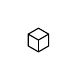
\begin{tikzpicture}[scale=0.15, baseline=-0.5ex]
        % Define the precise value for horizontal distance
        \pgfmathsetmacro{\hdist}{sqrt(3)/2}

        % Symmetric hexagon
        \draw (0,1) -- (\hdist,0.5) -- (\hdist,-0.5) -- (0,-1) -- (-\hdist,-0.5) -- (-\hdist,0.5) -- cycle;

        % Connect three non-consecutive vertices to the center
        \draw (0,0) -- (0,-1);
        \draw (0,0) -- (\hdist,0.5);
        \draw (0,0) -- (-\hdist,0.5);
    \end{tikzpicture}
}





\begin{document}

\setbeamertemplate{background}{
\includegraphics[]{img/Background.png}} 

%\renewcommand{\thefootnote}{\fnsymbol{footnote}}


\title[\href{https://arxiv.org/abs/2402.15892}{Statistical Games}]{\href{https://arxiv.org/abs/2402.15892}{Statistical Games} \\ {\small Playful approach to statistics}}
\author{\href{https://konczer.github.io/}{József Konczer}}
\date{3. May 2024}

\begin{frame}
\titlepage
\end{frame}




%\begin{frame}{Overview}
%\end{frame}

\section{Introduction}

\begin{frame}{Why? Mathematician Answer:}

\begin{itemize}
    \item Why not?
    \item It might appeal to some.
    \item In the first part, established concepts:
    \begin{itemize}
        \item Elementary calculations resulting sometimes surprising results.
    \end{itemize}
    \item Can be continued to:
    \begin{itemize}
        \item Optimization in Functional (Measure) spaces,
        \item Delicate tools, expansions, inequalities for exploring limiting cases,
        \item Quantum generalization (scenarios to quantum states).
    \end{itemize}
    \item + Fun to design concepts and notation, grounded by their ability to simplify proofs and calculations.
\end{itemize}



\end{frame}


\begin{frame}{Why? Philosophical Answer:}

\begin{columns}

% Column 2    
\begin{column}{0.5\textwidth}
    \begin{figure}
    \centering
        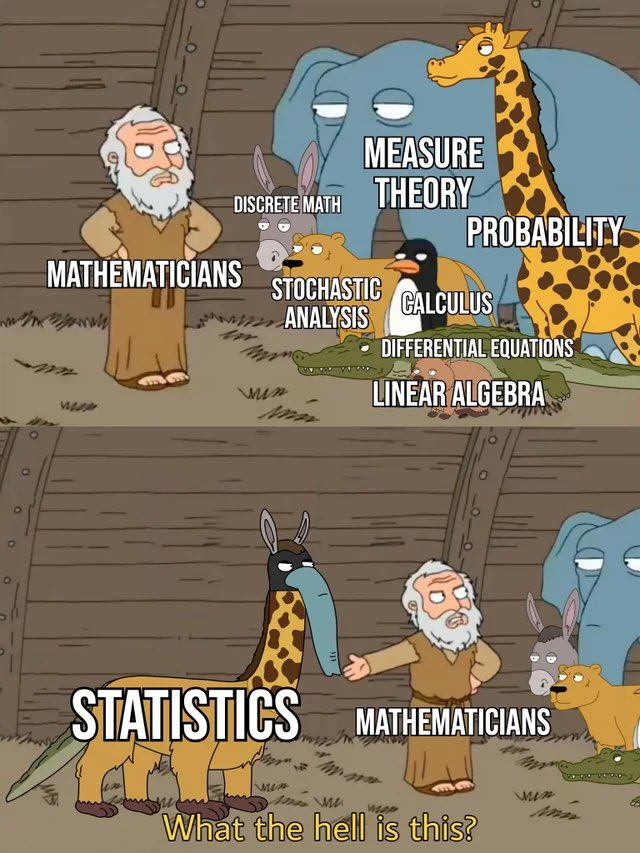
\includegraphics[width=0.75\textwidth]{img/StatisticsMeme.jpeg}
        \caption{\small from \href{https://twitter.com/miniapeur/status/1673275056812597248/photo/1}{@miniapeur} on $\mathbb{X}$}
    \end{figure}
\end{column}

        % Column for the text
        \begin{column}{0.5\textwidth}
            \begin{itemize}
    \item Pursuit for simplicity$^*$ and coherence.
    \begin{itemize}
        \item * in thought, not necessarily in techniques.
    \end{itemize}
    \item Searching for an organizing principle in Statistics.
    \item Formalization and (re-)introduction of Uncertainty.
    \item Epistemology $\to$ Strategy.
    \item Prior $\to$ Fictional Player.
\end{itemize}
        \end{column}

\end{columns}

\end{frame}


\begin{frame}{Oversimplified introduction to Game Theory}

\begin{wrapfigure}{r}{0\textwidth}
    \centering
    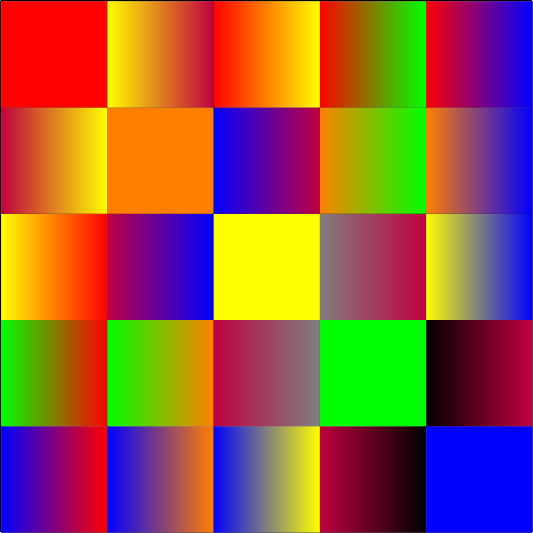
\includegraphics[width=0.2\textwidth]{img/GameTheoryLogo.png}
    \caption{\tiny \centering \href{https://nordstrommath.com/IntroGameTheoryv4-2020.pdf}{Introduction to Game Theory} by J. F. Nordstrom}
\end{wrapfigure}

Action sets for 2 Players: $\mathcal{A}_1, \mathcal{A}_2$.

Utility matrices:

\[
    \mathcal{A}_1 \times \mathcal{A}_2 \mapsto \mathcal{C}, \ 
    \begin{cases}
    u_1 : \mathcal{C} \mapsto \mathbb{R}, \text{or } (\mathcal{A}_1 \times \mathcal{A}_2 \mapsto \mathbb{R}) \\
    u_2 : \mathcal{C} \mapsto \mathbb{R}, \text{or } (\mathcal{A}_1 \times \mathcal{A}_2 \mapsto \mathbb{R})
\end{cases}
\]

Strategies:

\[
\sigma_1 \in \mathscr{P}(\mathcal{A}_1), \quad
\sigma_2 \in \mathscr{P}(\mathcal{A}_2)
\]

Expected utilities: $EU_i = \mathbb{E}_{\alpha_1 \sim \sigma_1, \alpha_2 \sim \sigma_2}[u_i(\alpha_1,\alpha_2)]$

\[
EU_1(a_1,\sigma_2) = \mathbb{E}_{\alpha_2 \sim \sigma_2}[u_i(a_1,\alpha_2)], \ 
EU_2(\sigma_1,a_2) = \mathbb{E}_{\alpha_1 \sim \sigma_1}[u_i(\alpha_1,a_2)]
\]

\end{frame}

\begin{frame}{Oversimplified introduction to Game Theory}

\begin{wrapfigure}{r}{0\textwidth}
    \centering
    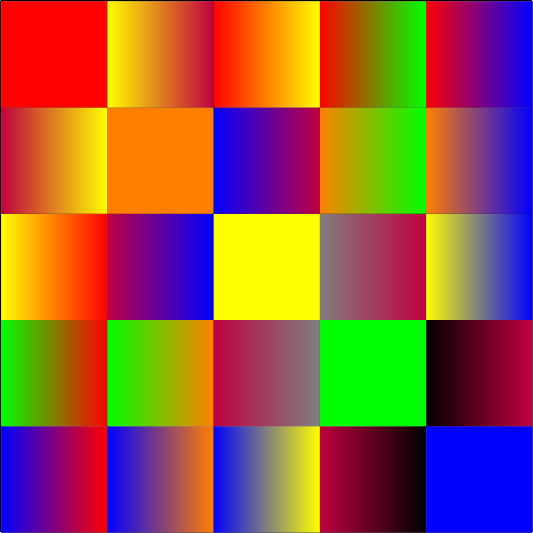
\includegraphics[width=0.2\textwidth]{img/GameTheoryLogo.png}
    \caption{\tiny \centering \href{https://nordstrommath.com/IntroGameTheoryv4-2020.pdf}{Introduction to Game Theory} by J. F. Nordstrom}
\end{wrapfigure}

Nash equilibrium is a strategy profile:

\[
\sigma^* = (\sigma_1^*,\sigma_2^*)
\]

Where no player’s expected utility can be improved by changing one’s own strategy.

\[
\begin{split}
    \forall a_1 \in \mathcal{A}_1, \  EU_1 \ge EU_1(a_1,\sigma_2^*) \\
    \forall a_2 \in \mathcal{A}_2, \  EU_2 \ge EU_2(\sigma_1^*,a_2)
\end{split}
\]



Nash equilibrium always exist (for finite action sets), but it is not necessarily unique.

\end{frame}


\section{Fisher \& Bayesian games}

\subsection{Fisher games}

\begin{frame}{}

\begin{definition}[Fisher game]
\label{def:FisherGame}
There are two players, \PI/ (Guesser) and \PII/ (Chooser).
\PII/ needs to choose between scenario A or B first and then produce a binary sequence of length $M$ containing precisely $K_A$ or $K_B$ number of $1$-s. (Without losing generality, we will assume $K_A \le K_B$.)
Following this, \PI/ (not knowing the actions of \PII/) can sample $N$ number of bits, and after observing their value, she guesses scenario A or B.

If \PI/ guessed the scenario correctly, she wins the game (\textcolor{w}{$\blacksquare$}) and loses otherwise (\textcolor{l}{$\blacksquare$}). 
The above-defined Fisher game will be denoted as 
\G{N, K_A, K_B, M}.

\end{definition}


\end{frame}


\begin{frame}[shrink=30]



\begin{gametable}[H]
\captionsetup{justification=centering}
\caption{\label{game:GeneralFisherGame} General description of \\ \G{N, K_A, K_B, M}}
\centering
\begin{tabularx}{0.73\textwidth}{ X | X }
\hline
 &  \\
\multicolumn{1}{c|}{\PI/} & \multicolumn{1}{c}{\PII/} \\
 &
\begin{itemize}
        \item Chooses scenario A or B,
        \begin{itemize}
            \item then chooses a binary sequence available for the chosen scenario.
        \end{itemize}
\end{itemize}
\\
\begin{itemize}
        \item Chooses $N$ indices for sampling,
        \begin{itemize}
            \item based on the bits in the chosen sample, guesses scenario A or B.
        \end{itemize}
    \end{itemize}
& \\
& \\
\multicolumn{2}{c}{
    \begin{minipage}{0.5\linewidth}
        \centering
        If \PI/ guessed the scenario correctly, she wins the game (\textcolor{w}{$\blacksquare$}) and loses otherwise (\textcolor{l}{$\blacksquare$}).
    \end{minipage}
} \\
\end{tabularx}
\end{gametable}


\end{frame}




\begin{frame}{Statistically trivial example (Matching Pennies)}

\G{N=0,K_A=0,K_B=0,M=0}:

\begin{equation*}
u_1=
\begin{bmatrix}
\wbox & \lbox \\
\lbox & \wbox
\end{bmatrix}, \quad
u_2=
\begin{bmatrix}
\lbox & \wbox \\
\wbox & \lbox
\end{bmatrix}
\end{equation*}

\pause

\begin{figure}[H]
    \centering
    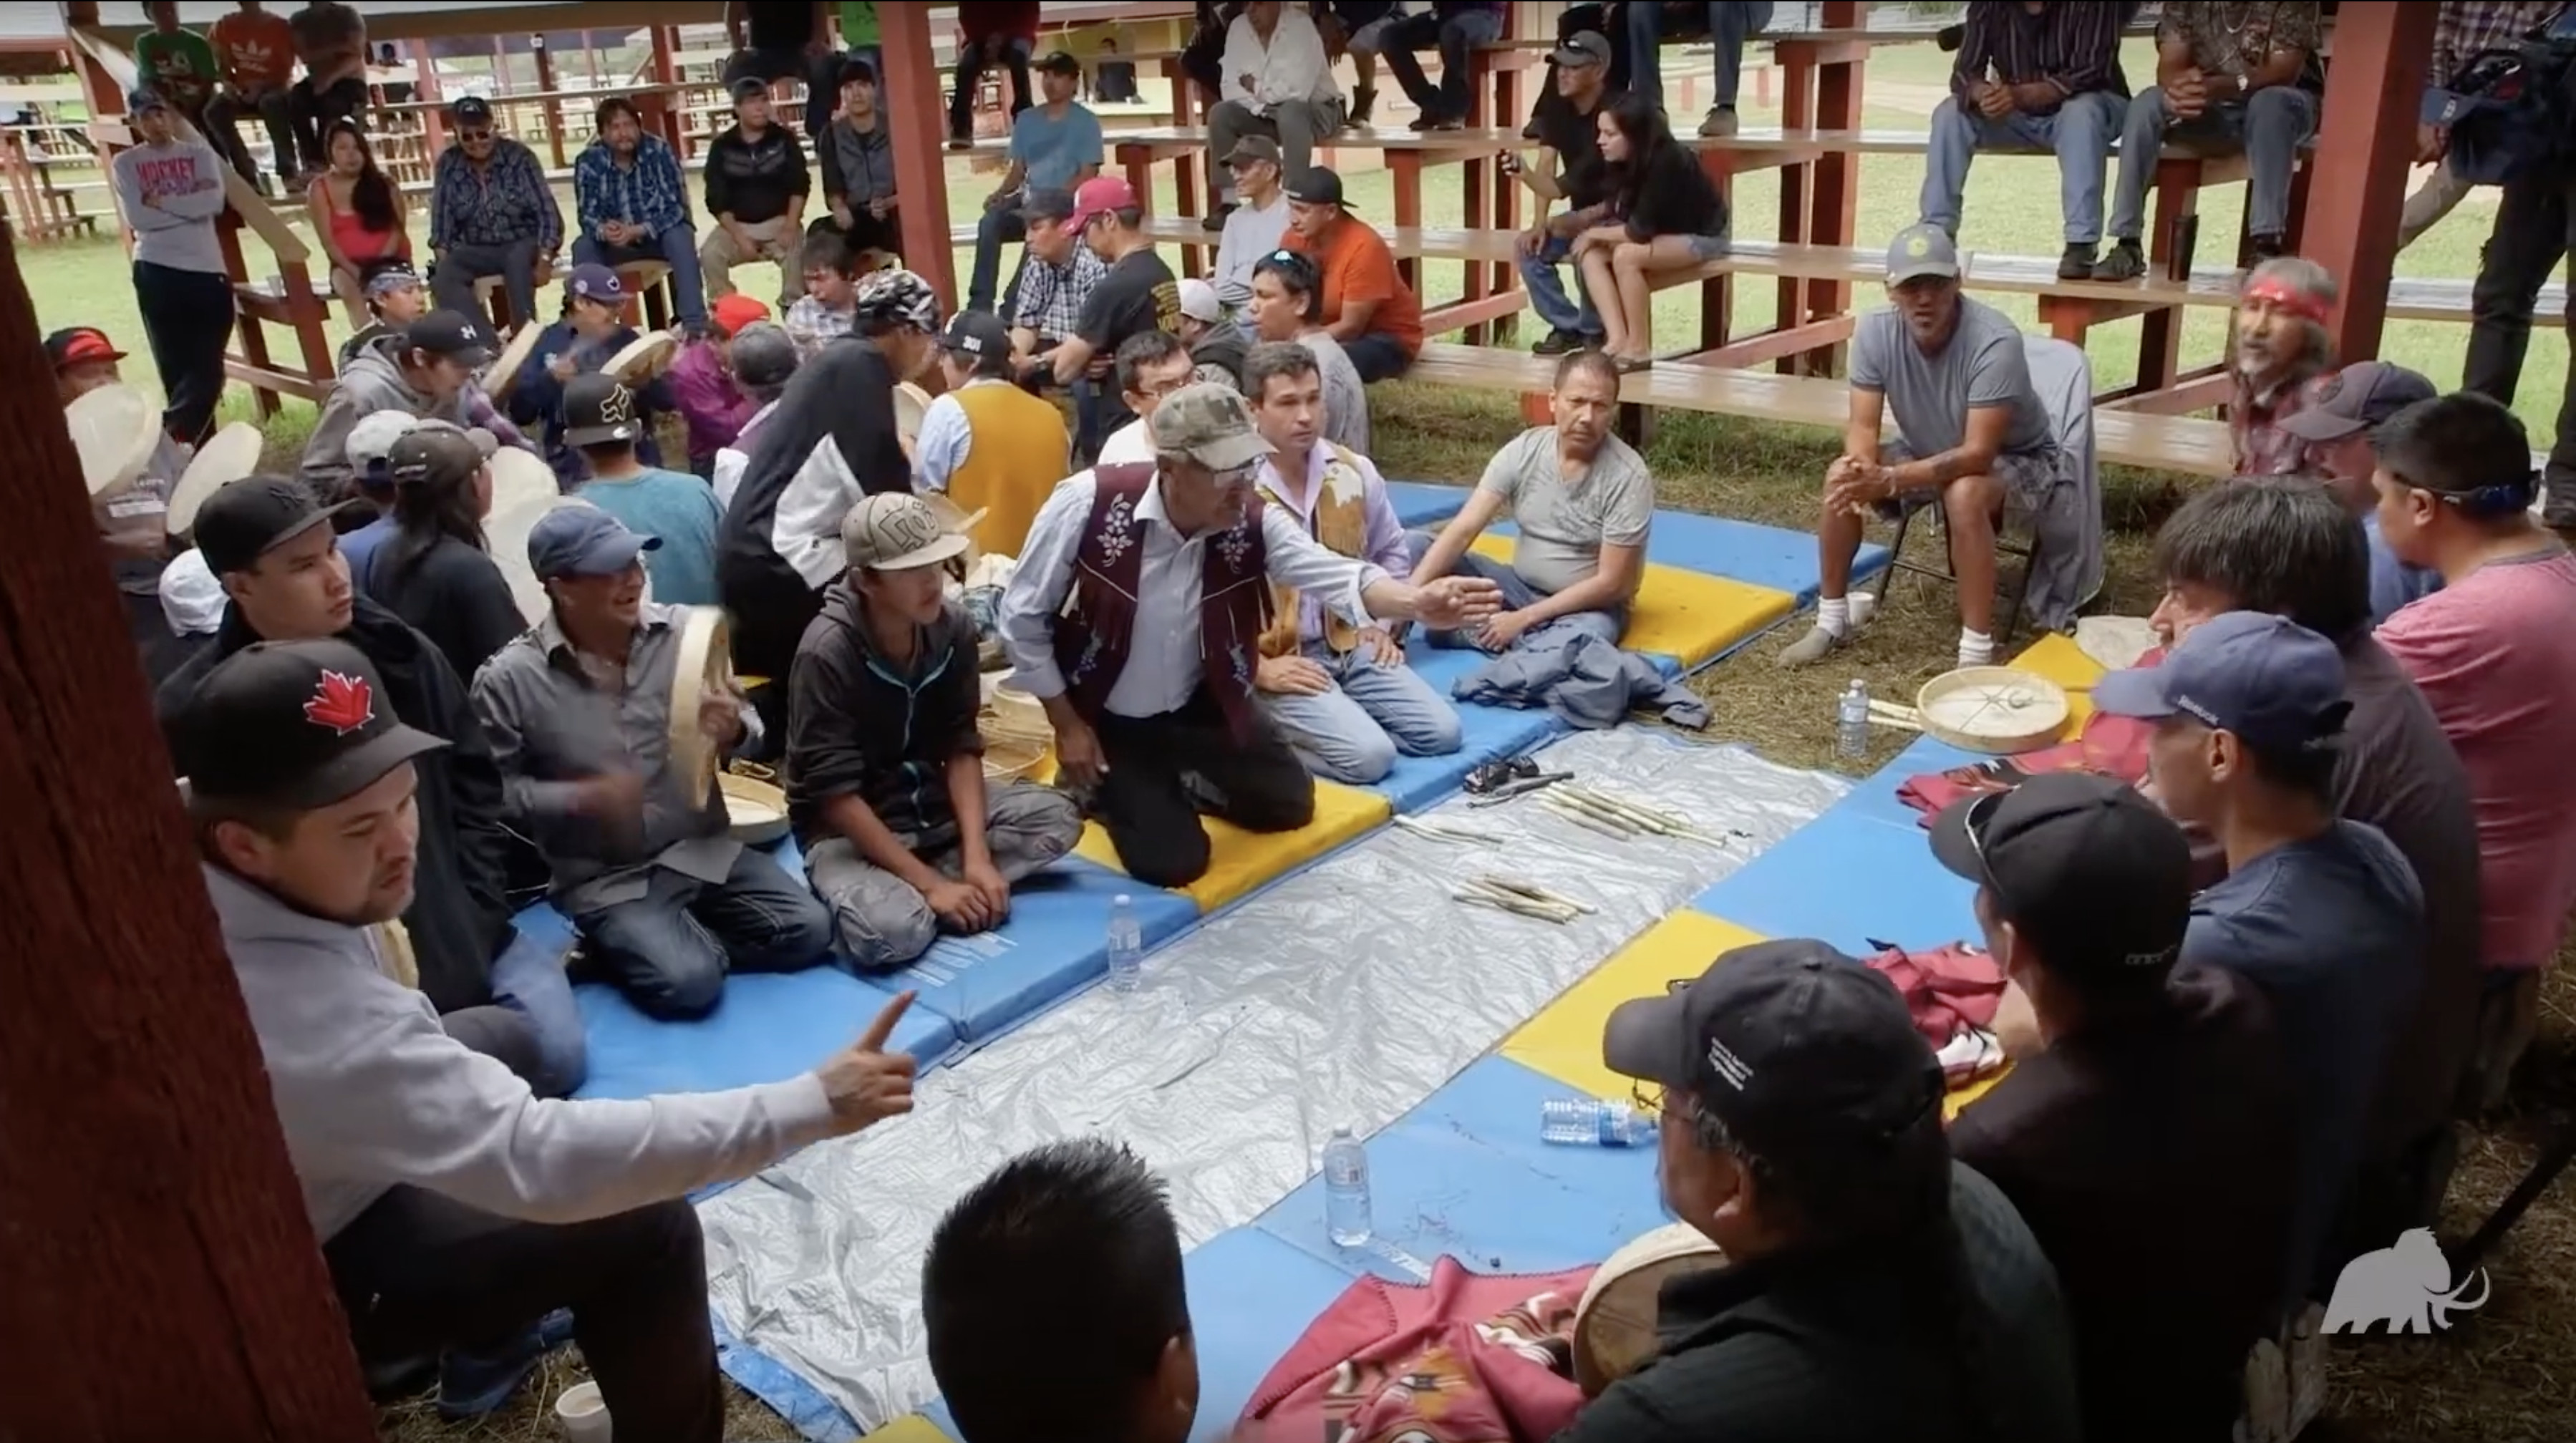
\includegraphics[width=0.65\textwidth]{img/HandGame.jpg}
    \caption{\small \href{https://www.youtube.com/watch?v=IgznW43DLbg}{Hand Game}}
    \label{fig:HandGame}
\end{figure}

\end{frame}

\begin{frame}{Statistically trivial example (Matching Pennies)}

The game has one unique Nash equilibrium: the players are guessing/choosing
A or B with an equal $50\%$ chance, and both players have a $50\%$ chance to win or lose.

\[
\sigma_1^* = (1/2,1/2), \quad \sigma_2^* = (1/2,1/2)
\]

\[
v^* = 1/2
\]

\end{frame}

\begin{frame}{Smallest nontrivial case}
\G{N=1,K_A=0,K_B=1,M=2}:

\begin{equation*}
    \label{eq:SimplestFisher_A2}
    \mathcal{A}_2 = \{ (A, (\wb,\wb)), (B, (\wb,\bb)) ,(B,(\bb,\wb)) \}
\end{equation*}

\begin{equation*}
\begin{split}
\mathcal{A}_1' = \{ 
& (1,\{(\wb) \to A, (\bb) \to B\}), (1,\{(\wb) \to B, (\bb) \to B\}), \\
& (2,\{(\wb) \to A, (\bb) \to B\}), (2,\{(\wb) \to B, (\bb) \to B\})
\}
\end{split}
\end{equation*}

\pause

\begin{equation*}
    \label{eq:SimplestFisherComplete}
    \underline{\sigma}'^*_1(\lambda)=(1/3,\lambda/3,1/3,(1-\lambda)/3), \quad \underline{\sigma}'^*_2(\lambda)=(1/3,1/3,1/3), 
\end{equation*}

\begin{equation*}
    \underline{\sigma}'^{\text{\ding{100}}}_1 = 
    \underline{\sigma}'^{*S}_1=(1/3,1/6,1/3,1/6), \quad 
    \underline{\sigma}'^{\text{\ding{100}}}_2 =
    \underline{\sigma}'^{*S}_2=(1/3,1/3,1/3)
\end{equation*}

\end{frame}

\begin{frame}[shrink=35]

\begin{gametable}[H]
\captionsetup{justification=centering}
\caption{\label{game:1_2_1_2} Symmetric equilibrium strategy for \\ \G{N=1, K_A=0, K_B=1, M=2}}
\centering
\begin{tabularx}{0.73\textwidth}{ X | X }

\hline
 &  \\
\multicolumn{1}{c|}{\PI/} & \multicolumn{1}{c}{\PII/} \\
 &
\begin{itemize}
        \item Choose scenario A with probability $1/3$, and scenario B with probability $2/3$
        \begin{itemize}
            \item Choose uniformly from all different allowed sequences.
        \end{itemize}
\end{itemize}
\\
\begin{itemize}
        \item Sample randomly from all possible indices uniformly
        \begin{itemize}
            \item in case the sampled bit is $\wb$:
            \begin{itemize}
                \item guess A with probability $2/3$
                \item and B with probability $1/3$ 
            \end{itemize}
            \item in case the sampled bit is $\bb$:
            \begin{itemize}
                \item guess B
            \end{itemize}
        \end{itemize}
    \end{itemize}
& \\
\end{tabularx}
\end{gametable}


\end{frame}

\begin{frame}{}

\begin{figure}[H]
    \centering
    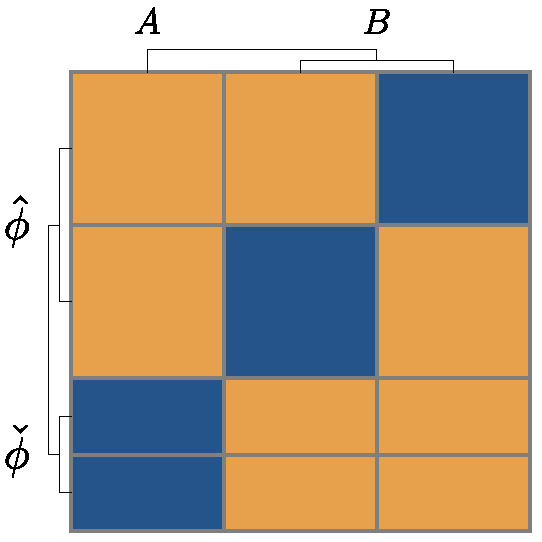
\includegraphics[width=6 cm]{img/StrategyPlot_1012.pdf}
    \caption{\small \centering Strategy plot for the symmetric equilibrium of \G{N=1,K_A=0,K_B=1,M=2}.}
    \label{fig:StrategyPlot_1012}
\end{figure}

\end{frame}

\begin{frame}[shrink=40]{Ansatz}

\begin{gametable}[H]

\captionsetup{justification=centering}
\caption{\label{game:Ansatz1} {\bf Ansatz} for the general \G{N, K_A, K_B, M} case, \\ having 3 free variables: $P$, $k^\bullet$ and $\nu$:}

\centering
\begin{tabularx}{0.73\textwidth}{ X | X }

\hline
 &  \\
\multicolumn{1}{c|}{\PI/} & \multicolumn{1}{c}{\PII/} \\
 &
\begin{itemize}
        \item choose scenario A with probability $\pi(\mathrm{A})=P$, or B with probability $\pi(\mathrm{B})=1-P$.
        \begin{itemize}
            \item Choose uniformly from all different allowed sequences.
        \end{itemize}
    \end{itemize}
\\
 \begin{itemize}
        \item sample $N$ bits randomly and uniformly from all available $M$ bits,
        \begin{itemize}
            \item in case the number of $\bb$-s $k < k^\bullet$ guess A,
            \item in case $k=k^\bullet$:
            \begin{itemize}
                \item guess A with probability $\mu(\hat{\phi}) = \nu$,
                \item guess B with probability $\mu(\check{\phi}) = 1-\nu$,
            \end{itemize}
            \item in case the number of $\bb$-s $k > k^\bullet$ guess B.
        \end{itemize}
    \end{itemize}
& \\
\end{tabularx}
\end{gametable}


\end{frame}

\begin{frame}[shrink=10]{}

\begin{theorem}[Symmetrical equilibrium]

The parameters $(k^*, \nu^*, P^*)$ can be determined from the parameters of the game $(N, K_A, K_B, M)$:

\begin{equation}
    \label{thm:SymEqHypergeom}
    p_k(A) = \frac{\binom{K_A}{k} \binom{M-K_A}{N-k}}{\binom{M}{N}}, \quad
    p_k(B) = \frac{\binom{K_B}{k} \binom{M-K_B}{N-k}}{\binom{M}{N}}
\end{equation}

\begin{equation}
    \label{thm:Fisher_Ps}
    P^* = \frac{p_{k^*}(B)}{p_{k^*}(A)+p_{k^*}(B)}
\end{equation}

\begin{equation}
    \label{thm:SymEqNu}
    \nu^* = \frac{\sum_{k \ge k^*} p_k(B) - \sum_{k < k^*} p_k(A)}{p_{k^*}(A)+p_{k^*}(B)}
\end{equation}

Finally, $k^*$ is the smallest integer, for which the sum of probabilities becomes greater than $1$:

\begin{equation}
    \label{thm:Fisher_ks}
    \sum_{k \le k^*} p_k(A)+p_k(B) > 1, \quad \mathrm{while} \quad \sum_{k<k^*} p_k(A)+p_k(B) \le 1
\end{equation}

\end{theorem}

\end{frame}

\begin{frame}{}

\begin{figure}[H]
    \centering
    \begin{subfigure}[b]{0.45\textwidth}
        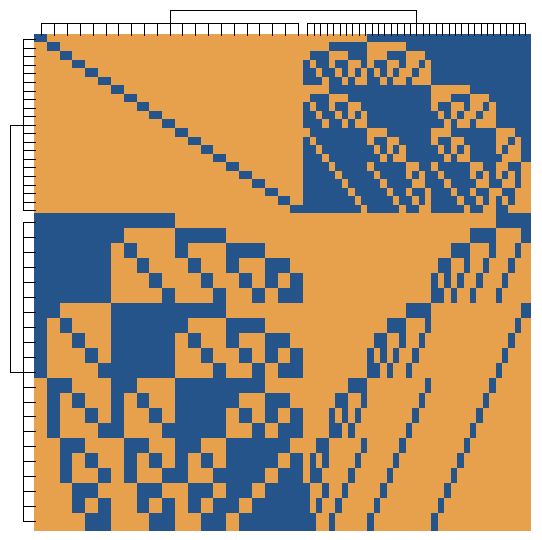
\includegraphics[width=\textwidth]{img/StrategyPlot_2_2_4_7.pdf}
        \caption{\small \centering \G{N=2,K_A=2,K_B=4,M=7}}
        \label{fig:StrategyPlot_G_2_2_4_7}
    \end{subfigure}
    \hspace{0.05\textwidth} % space between images
    \begin{subfigure}[b]{0.45\textwidth}
        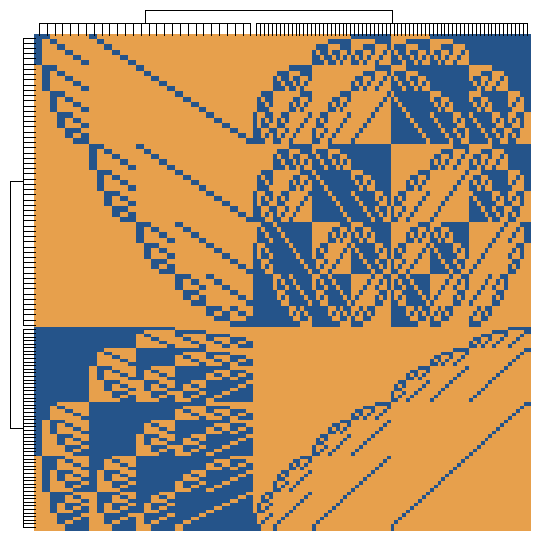
\includegraphics[width=\textwidth]{img/StrategyPlot_3_2_4_8.pdf}
        \caption{\small \centering \G{N=3,K_A=2,K_B=4,M=8}}
        \label{fig:StrategyPlot_G_3_2_4_8}
    \end{subfigure}
    \caption{\small \centering Strategy plots for symmetric equilibria}
    \label{fig:StrategyPlots}
\end{figure}


\end{frame}

\begin{frame}{}

\begin{figure}[H]
    \centering
    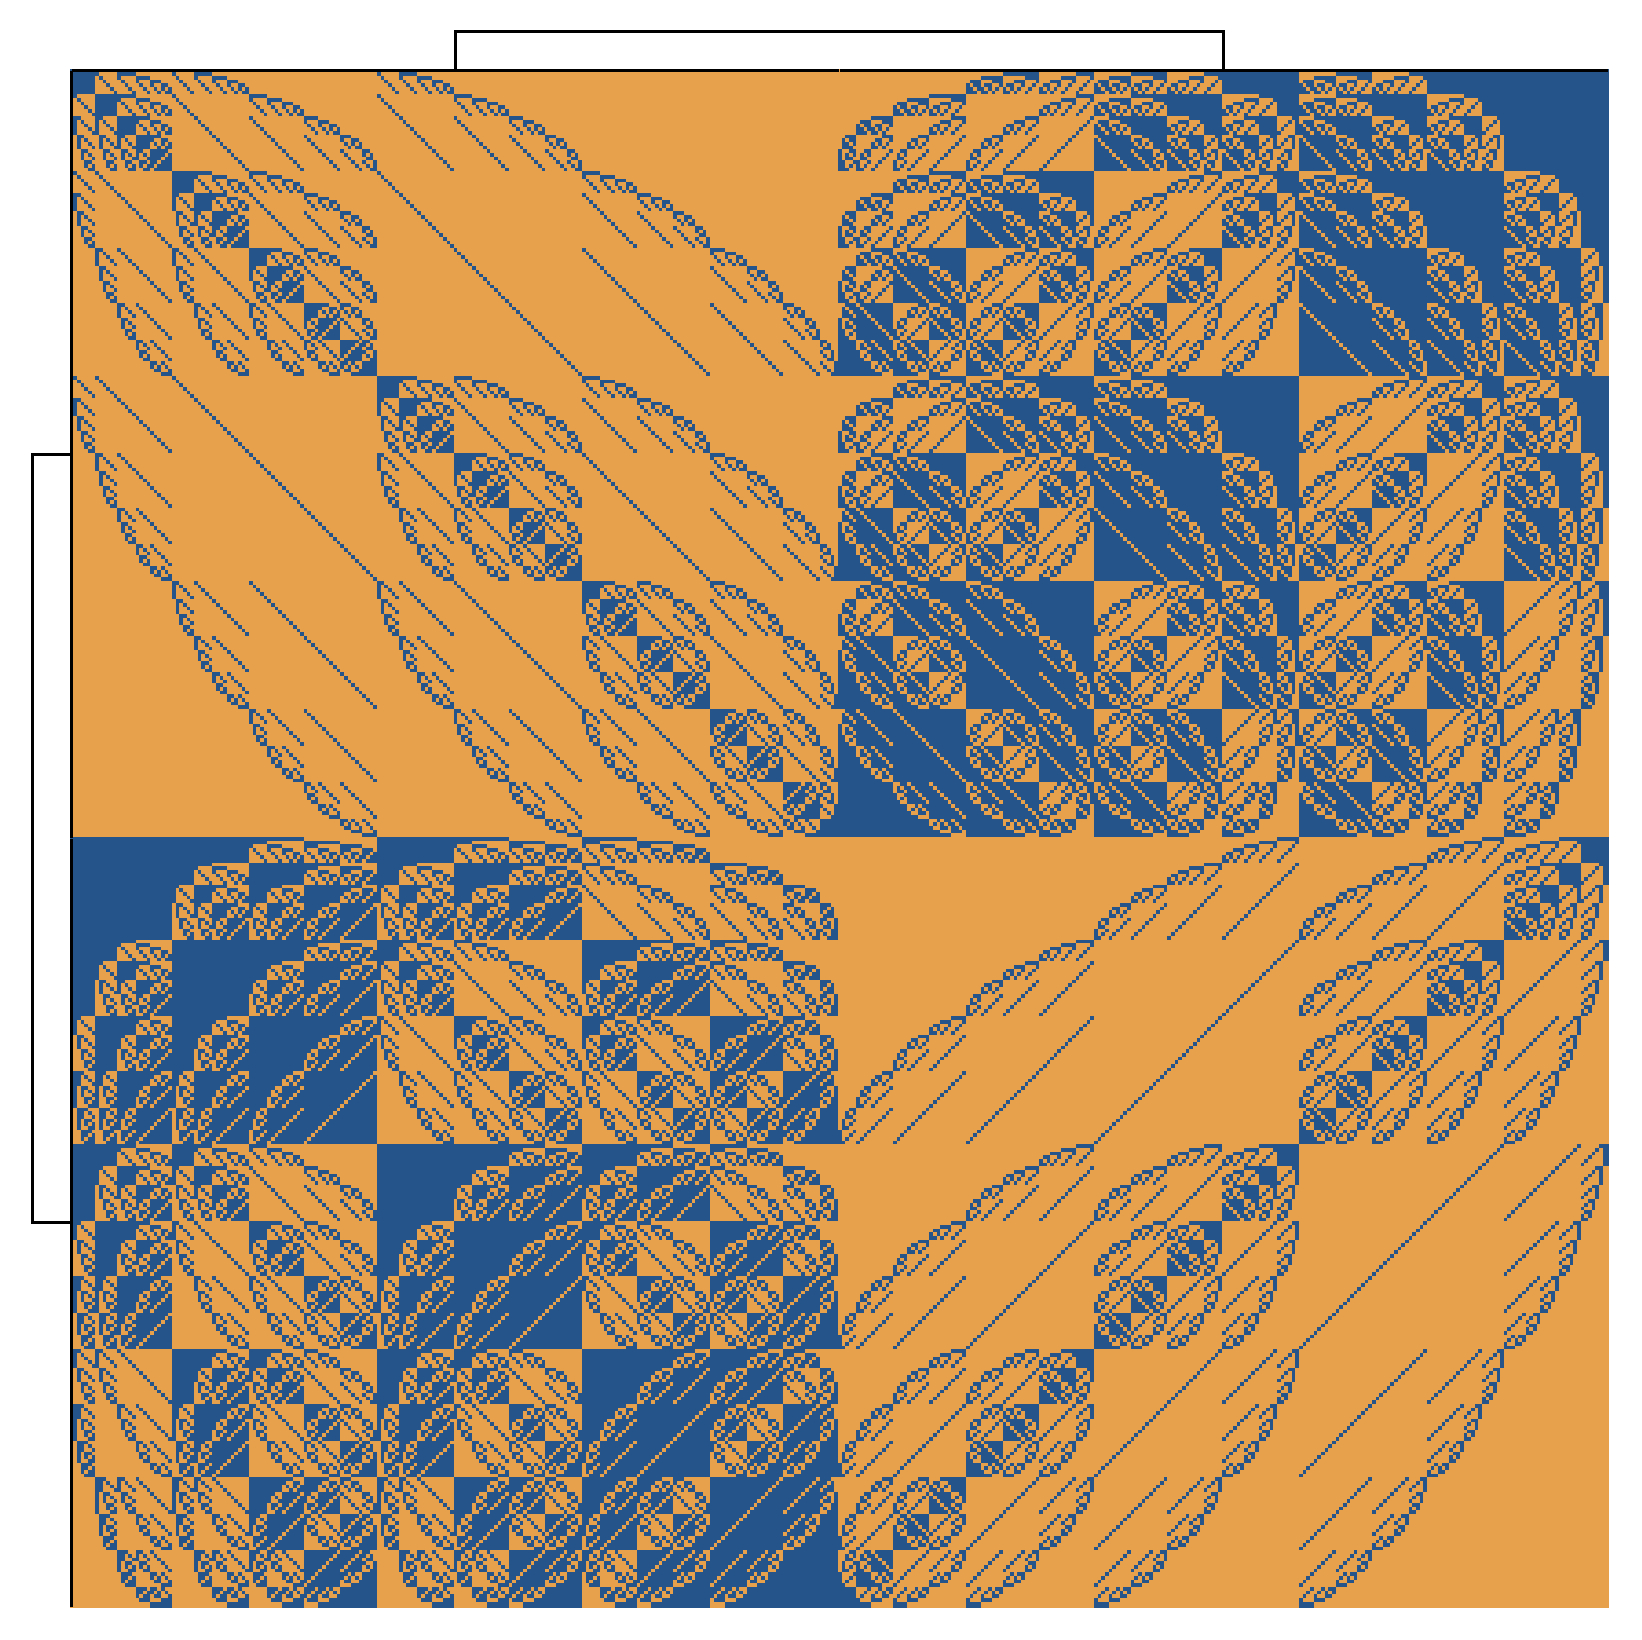
\includegraphics[width=0.6\textwidth]{img/StrategyPlot_4_4_6_10.pdf}
    \caption{\small \centering Strategy plot for the symmetric equilibrium of \G{N=4,K_A=4,K_B=6,M=10}.}
    \label{fig:StrategyPlot_G_4_4_6_10}
\end{figure}

\end{frame}

\begin{frame}[shrink=40]

\begin{figure}[H]
    \centering
    \begin{subfigure}[b]{0.3\textwidth}
        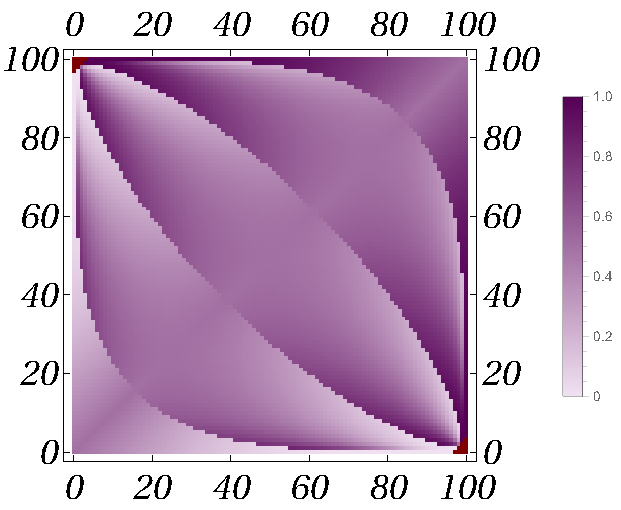
\includegraphics[width=\textwidth]{img/P_Plot_4_100.pdf}
        \caption{\small \centering $P^*(K_A,K_B)$}
        \label{fig:Game4__100_P}
    \end{subfigure}
    \hfill % space between images
    \begin{subfigure}[b]{0.3\textwidth}
        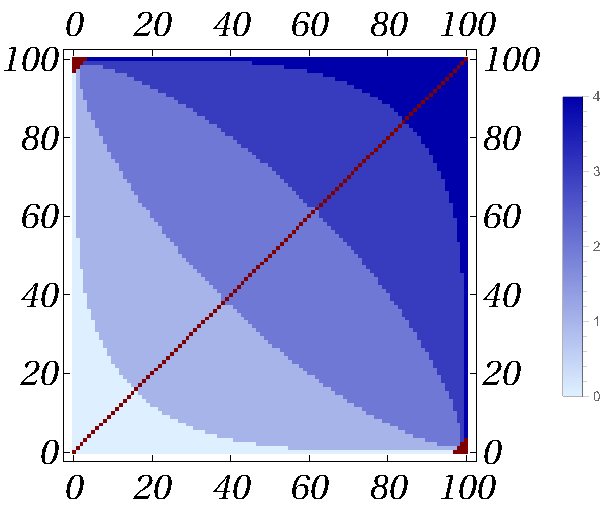
\includegraphics[width=\textwidth]{img/k_Plot_4_100.pdf}
        \caption{\small \centering $k^*(K_A,K_B)$}
        \label{fig:Game4__100_k}
    \end{subfigure}
    \hfill % space between images
    \begin{subfigure}[b]{0.3\textwidth}
        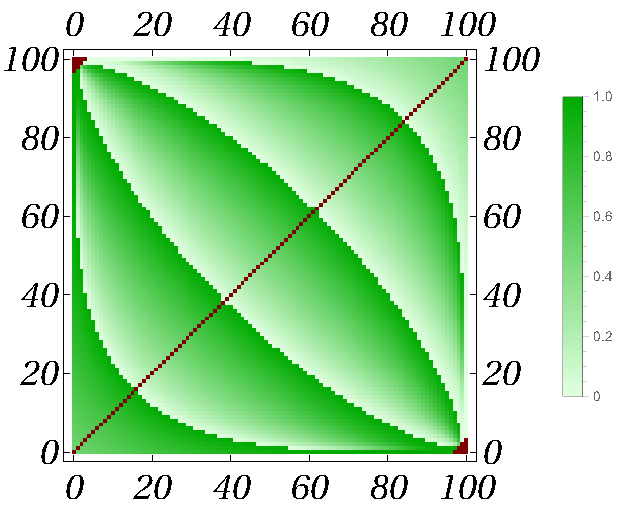
\includegraphics[width=\textwidth]{img/nu_Plot_4_100.pdf}
        \caption{\small \centering $\nu^*(K_A,K_B)$}
        \label{fig:Game4__100_nu}
    \end{subfigure}
    
    \caption{\G{N=4,K_A,K_B,M=100}}
    \label{fig:Game4__100_Pknu}
\end{figure}


\begin{figure}[H]
    \centering
    \begin{subfigure}[b]{0.3\textwidth}
        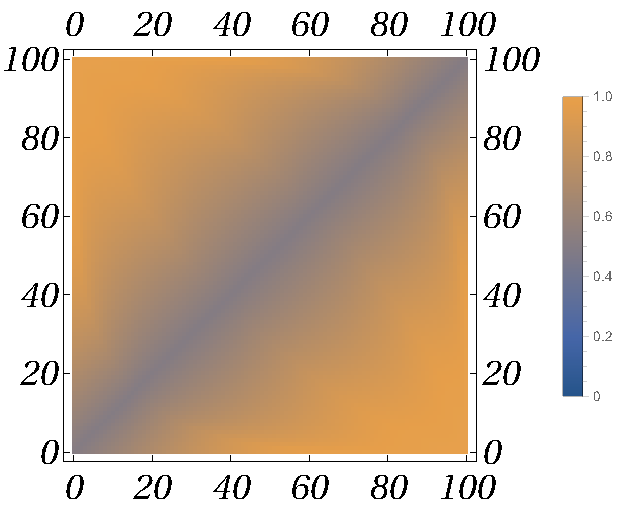
\includegraphics[width=\textwidth]{img/v_Plot_4_100.pdf}
        \caption{\small \centering $v^*(K_A,K_B)$}
        \label{fig:Game4__100_v}
    \end{subfigure}
    \hspace{0.05\textwidth} % space between images
    \begin{subfigure}[b]{0.3\textwidth}
        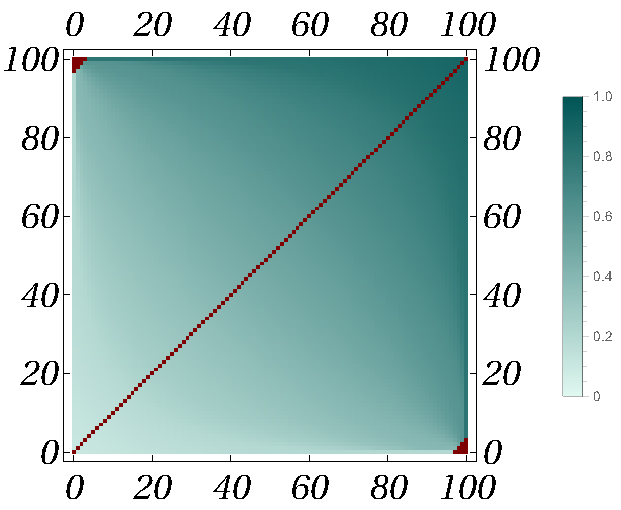
\includegraphics[width=\textwidth]{img/s_Plot_4_100.pdf}
        \caption{\small \centering $s^*(K_A,K_B)$}
        \label{fig:Game4__100_s}
    \end{subfigure}
    \caption{\G{N=4,K_A,K_B,M=100}}
    \label{fig:Game4__100_vs}
\end{figure}



\end{frame}

\begin{frame}{Emerged Statistical concepts}


\begin{columns}

\begin{column}{0.5\textwidth}
            
\begin{itemize}
    \item Sufficient statistics
    \item Type I and Type II errors
    \item Randomized sampling
    \item Emergence of probability distributions
    \item Randomized policies (appears here)
    \item Interpretation of mixed strategies (mostly appears here)
\end{itemize}
        \end{column}

% Column 2    
\begin{column}{0.5\textwidth}
    \begin{figure}
    \centering
        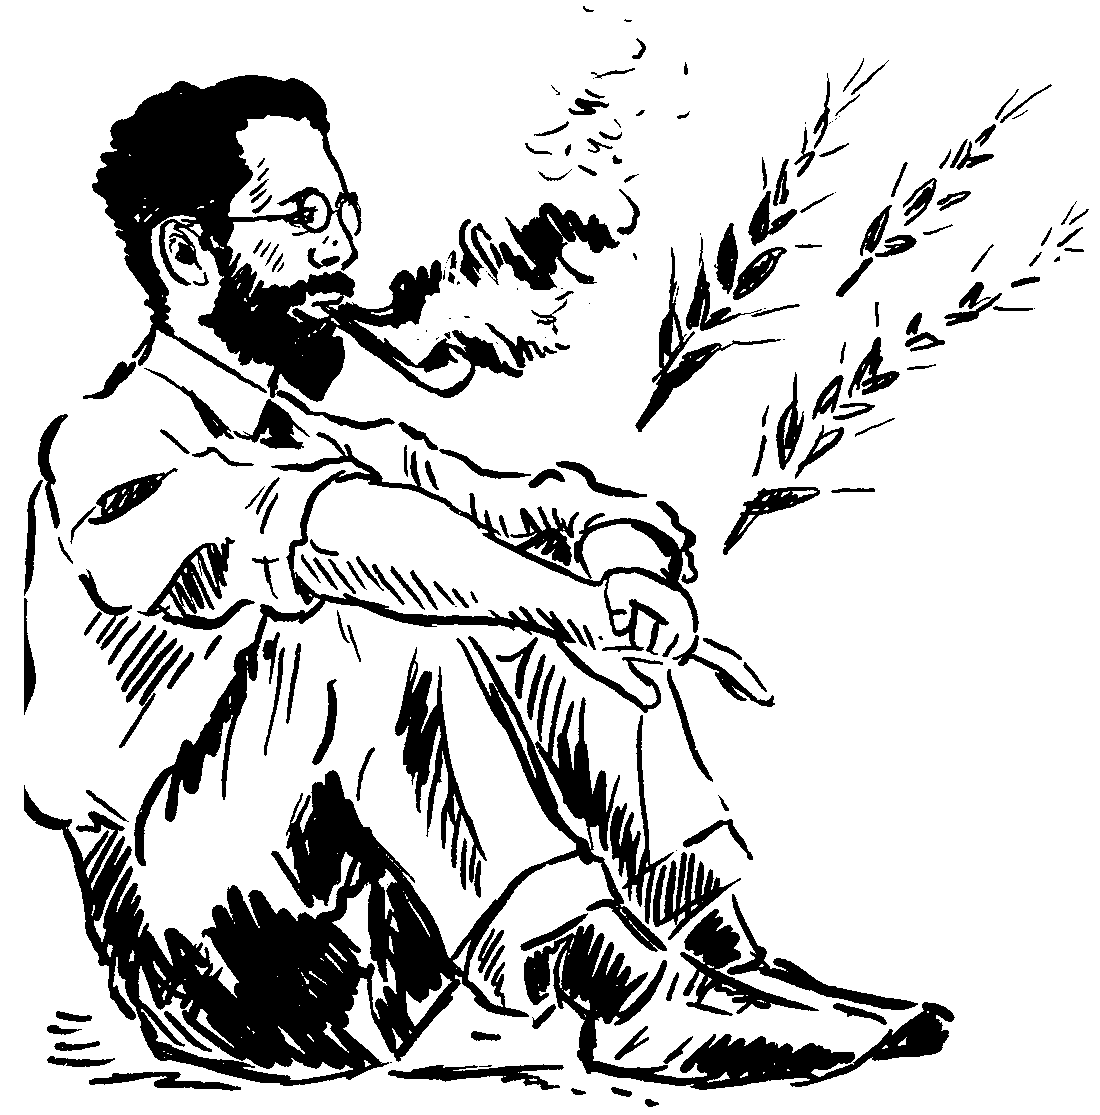
\includegraphics[width=0.75\textwidth]{img/RAFisher.png}
        \caption{\small \centering \href{https://statisticsblog.com/2012/01/15/r-a-fisher-illustration/}{R. A. Fisher illustration} by Rachelle Scarfó}
    \end{figure}
\end{column}
        

\end{columns}


\end{frame}

\begin{frame}{Type I and Type II errors}

    \begin{quote}
    We may now discuss what meaning could be given to the words:
    ``a test independent of the probability law a priori.''

    {\it
    Definition A. The phrase might be defined as implying a choice
    of critical region $w$ in such a way that the probability $P_\mathrm{Error}$ of
    making an error in testing $H_0$ had a value independent of the
    probabilities $\pi(A)$, $\pi(B)$.
    }

    \hfill --- Definition A in Neyman, Pearson 1933b \footnote{the notation has been slightly modified to harmonize with the notation used in this work}.
    \end{quote}
    
\end{frame}

\begin{frame}{Interpretation of mixed strategies}

    \begin{quote}
    {\it
    Mixed strategy can alternatively be viewed as the belief held by all other players concerning a player's actions. A mixed strategy equilibrium is then an $n$-tuple of common knowledge expectations, which has the property that all the actions to which a strictly positive probability is assigned are optimal, given the beliefs. A player's behavior may be perceived by all the other players as the outcome of a random device even though this is not the case.
    }
    
    \hfill --- Ariel Rubinstein 1991.
    \end{quote}
    
\end{frame}

\subsection{Bayesian games}

\begin{frame}{Bayesian betting}



\begin{columns}

\begin{column}{0.7\textwidth}
            
{\bf Double or nothing:}
Now, we enter a different casino, where instead of betting simply on scenario A or B, we can place some portion of our capital on each alternative. The portion we put on the winning scenario (chosen by \PII/) will be doubled, while the portion placed on the other scenario will be lost.

        \end{column}

% Column 2    
\begin{column}{0.3\textwidth}
    \begin{figure}
    \centering
        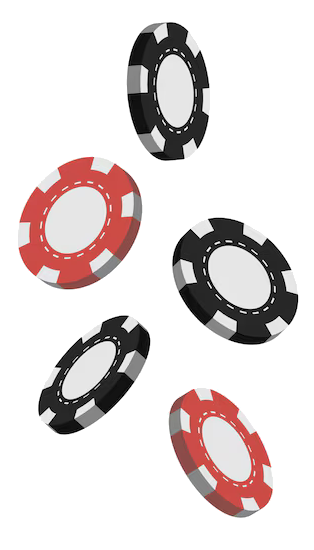
\includegraphics[width=0.8\textwidth]{img/Chips.png}
        \caption{\small \centering \href{https://www.freepik.com/premium-vector/casino-chips-falling-realistic-3d-gambling-poker-chips-background-poster-card-logo_19282474.htm}{Image source}}
    \end{figure}
\end{column}
        

\end{columns}

\end{frame}



\begin{frame}{}

\begin{definition}[Bayesian game]

There are two players, \PI/ and \PII/.
\PII/ needs to choose between scenario A or B, then produce a binary sequence of length $M$ containing precisely $K_A$ or $K_B$ number of $1$-s. (Without losing generality, we will assume $K_A \le K_B$.)
Following this, \PI/ (not knowing the actions of \PII/) can sample $N$ number of bits. After observing their values, she determines what portion of her capital $p'$ she places on scenario A (while the other $1-p'$ portion is placed on scenario B).

The portion \PI/ places on the scenario, chosen by \PII/, will be doubled, while the other part of her capital will be lost.
For this specific game, we will assume that \PI/ has a logarithmic utility function and that \PI/ and \PII/ are playing a zero-sum game.
The above-defined Bayesian game will be denoted as 
\BG{N, K_A, K_B, M}.

\end{definition}


\end{frame}

\begin{frame}[shrink=40]

\begin{gametable}[H]
\captionsetup{justification=centering}
\caption{\label{game:GeneralBayesianGame} General description of \\ \BG{N, K_A, K_B, M}}

\centering
\begin{tabularx}{0.73\textwidth}{ X | X }

\hline
 &  \\
\multicolumn{1}{c|}{\PI/} & \multicolumn{1}{c}{\PII/} \\
 &
\begin{itemize}
        \item Chooses scenario A or B,
        \begin{itemize}
            \item then chooses a binary sequence available for the chosen scenario.
        \end{itemize}
\end{itemize}
\\
\begin{itemize}
        \item Chooses $N$ indices for sampling,
        \begin{itemize}
            \item based on the bits in the chosen sample determines a continuous parameter $p' \in [0,1]$,
            \begin{itemize}
                \item and places her capital's $p'$ portion to scenario A and $1-p'$ portion to scenario B.
            \end{itemize}
        \end{itemize}
    \end{itemize}
& \\
& \\
\multicolumn{2}{c}{
    \begin{minipage}{0.75\linewidth}
        \centering
        The portion \PI/ places on the scenario chosen by \PII/ will be doubled, while the other part of her capital will be lost.
        
        \PI/ has a logarithmic utility function, \PI/ and \PII/ are playing a zero-sum game.
    \end{minipage}
} \\
\end{tabularx}
\end{gametable}


\end{frame}

\begin{frame}{}

\begin{figure}[H]
    \centering
    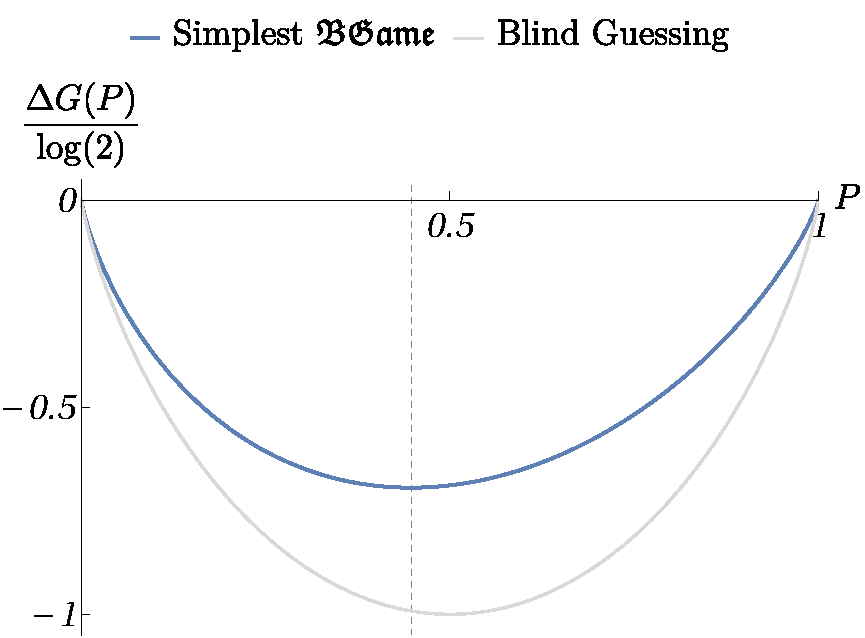
\includegraphics[scale=0.5]{img/G_BG_1_0_1_2.pdf}
    \caption{Visualization of the doubling factor difference (relative to a Sure winning game) $\Delta G(P)/\log(2)$ for \PI/ in the game: \BG{N=1,K_A=0,K_B=1,M=2} and a Blind guessing game, as a function of \PII/'s strategy of choosing A. The dashed grid line is placed to the equilibrium value of $P^*=1/\sqrt{5}$.}
    \label{fig:GainPlot1012}
\end{figure}

\end{frame}

\begin{frame}[shrink=20]
    \begin{theorem}[Bayesian equilibrium]
\label{thm:Bayesian}
\BG{N,K_A,K_B,M} has a unique Nash equilibrium, in which:

The parameters $(P^*, \{p'^*_k\})$ can be determined from the parameters of the game $(N, K_A, K_B, M)$:

\begin{equation}
    \label{thm:BayesEqHypergeom}
    p_k(A) = \frac{\binom{K_A}{k} \binom{M-K_A}{N-k}}{\binom{M}{N}}, \quad
    p_k(B) = \frac{\binom{K_B}{k} \binom{M-K_B}{N-k}}{\binom{M}{N}}
\end{equation}

\begin{equation}
    p'^*_k = \frac{P^* \ p_k(A)}{P^* \ p_k(A) + (1-P^*) \ p_k(B)}
\end{equation}

while $P^*$ is the unique minimum of the growth rate difference:

\begin{equation}
    \begin{split}
        \Delta G(P)=&P \ \sum_{k \in \mathbb{K}_A} p_k(A) \log \left ( \frac{P \ p_k(A)}{P \ p_k(A)+(1-P) \ p_k(B)} \right ) + \\
                    &(1-P) \ \sum_{k \in \mathbb{K}_B} p_k(B) \log \left ( \frac{(1-P) \ p_k(B)}{P \  p_k(A)+(1-P) \ p_k(B)} \right )
    \end{split}
\end{equation}



\end{theorem}

\end{frame}

\begin{frame}{Examples}

    \begin{figure}[H]
    \centering
    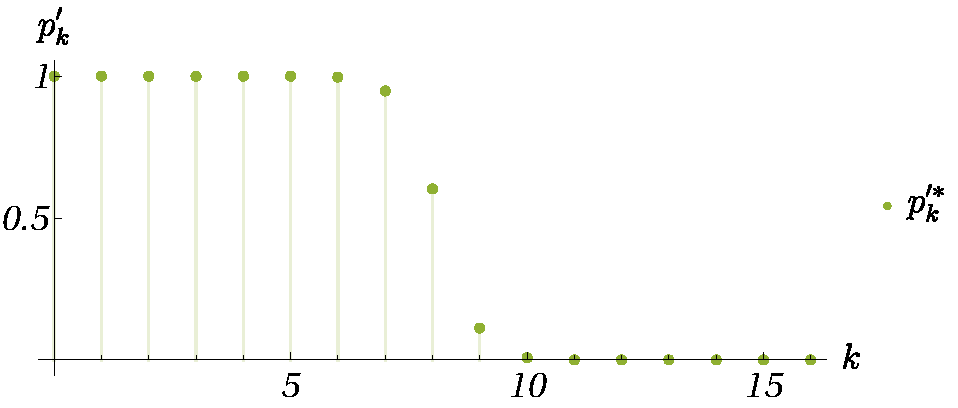
\includegraphics[scale=0.7]{img/ppkAB17_10_16_27.pdf}
    \caption{\small \centering Illustration of $p'^*_k$ for \BG{N=17,K_A=10,K_B=16,M=27}, in which case $P^*\approx 0.4953$.}
    \label{fig:ppkAB}
\end{figure}
    
\end{frame}

\begin{frame}[shrink=15]{Examples}
    \begin{figure}[H]
    \centering
    \begin{subfigure}[b]{0.3\textwidth}
        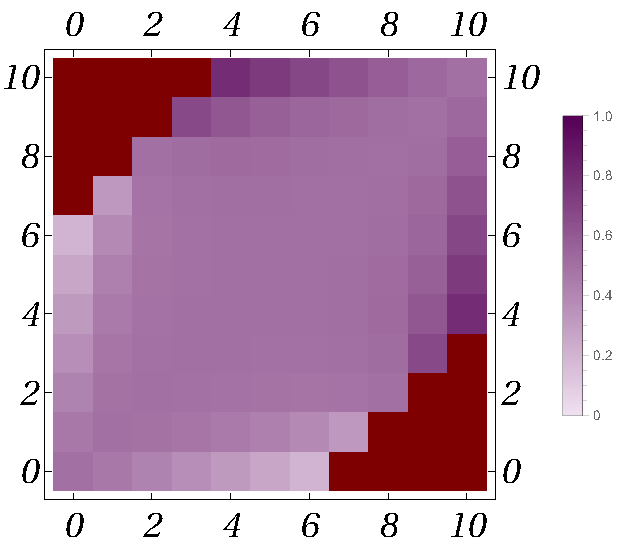
\includegraphics[width=\textwidth]{img/PB_Plot_4_10.pdf}
        \caption{\small \centering $P^*(K_A,K_B)$}
        \label{fig:BGame4_10_P}
    \end{subfigure}
    \hfill % space between images
    \begin{subfigure}[b]{0.3\textwidth}
        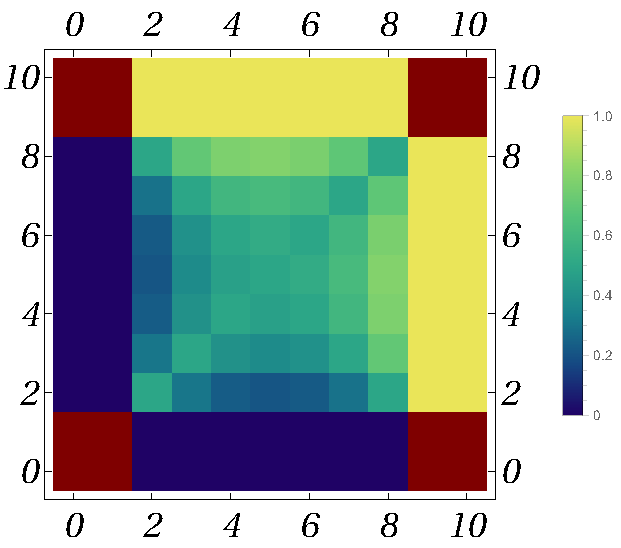
\includegraphics[width=\textwidth]{img/ppkB_Plot_4_10.pdf}
        \caption{\small \centering $p'^*_{k=2}(K_A,K_B)$}
        \label{fig:BGame4__10_ppk_2}
    \end{subfigure}
    \hfill % space between images
    \begin{subfigure}[b]{0.3\textwidth}
        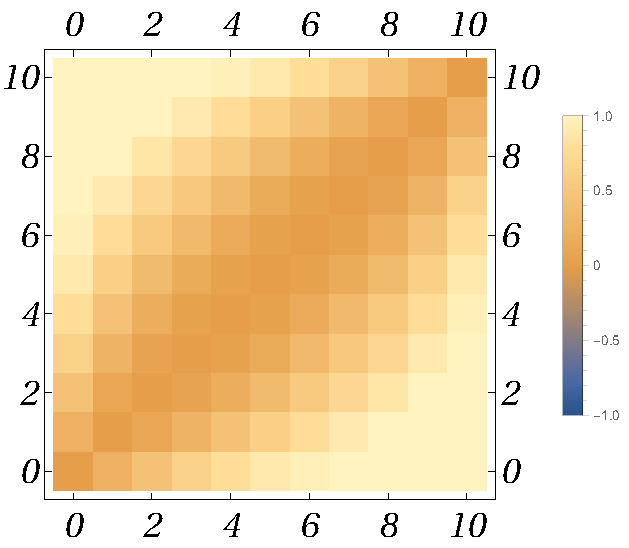
\includegraphics[width=\textwidth]{img/GB_Plot_4_10.pdf}
        \caption{\small \centering $G^*(K_A,K_B)/\log(2)$}
        \label{fig:BGame4__10_G}
    \end{subfigure}
    
    \caption{\small \centering \BG{N=4,K_A,K_B,M=10}}
    \label{fig:BGame4__10_PppkG}
\end{figure}
\end{frame}

\begin{frame}[shrink=10]{Examples}
    \begin{figure}[H]
    \centering
    \begin{subfigure}[b]{0.185\textwidth}
        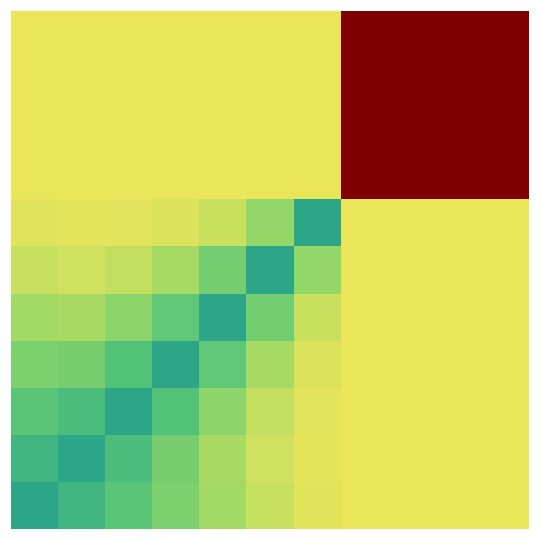
\includegraphics[width=\textwidth]{img/ppkB_Plot_4_0_10.pdf}
        \caption{$k=0$}
        \label{fig:ppkBG_4_0}
    \end{subfigure}
    \hspace{0.00\textwidth} % space between images
    \begin{subfigure}[b]{0.185\textwidth}
        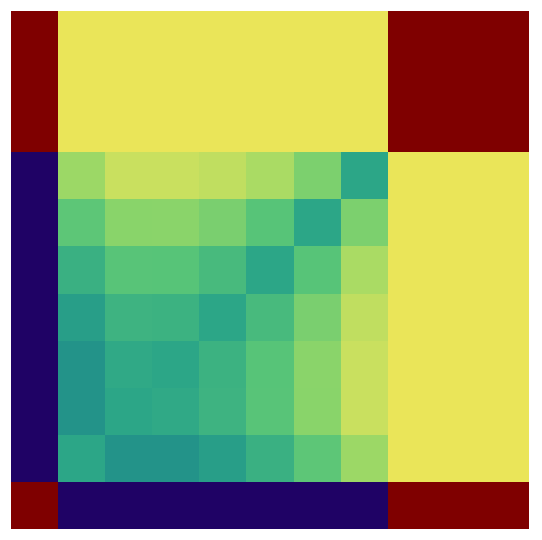
\includegraphics[width=\textwidth]{img/ppkB_Plot_4_1_10.pdf}
        \caption{$k=1$}
        \label{fig:ppkBG_4_1}
    \end{subfigure}
    \hspace{0.00\textwidth} % space between images
    \begin{subfigure}[b]{0.185\textwidth}
        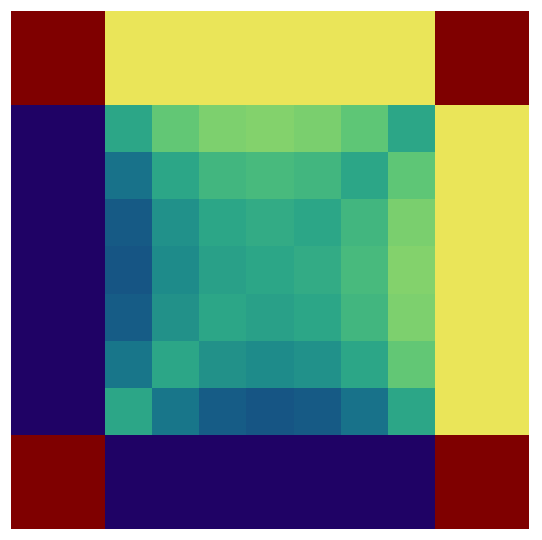
\includegraphics[width=\textwidth]{img/ppkB_Plot_4_2_10.pdf}
        \caption{$k=2$}
        \label{fig:ppkBG_4_2}
    \end{subfigure}
    \hspace{0.00\textwidth} % space between images
        \begin{subfigure}[b]{0.185\textwidth}
        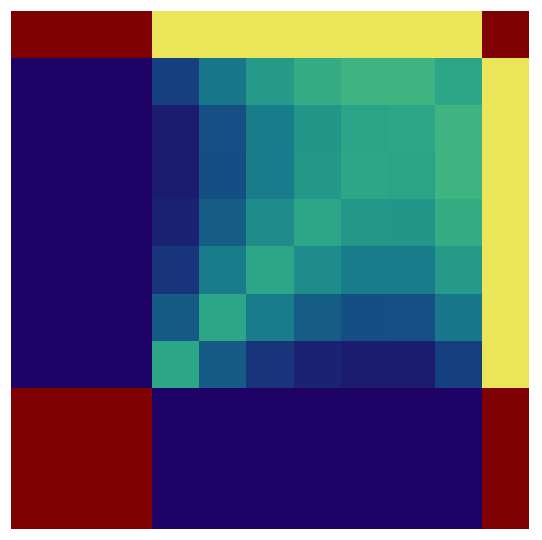
\includegraphics[width=\textwidth]{img/ppkB_Plot_4_3_10.pdf}
        \caption{$k=3$}
        \label{fig:ppkBG_4_3}
    \end{subfigure}
    \hspace{0.00\textwidth} % space between images
        \begin{subfigure}[b]{0.185\textwidth}
        
\includegraphics[width=\textwidth]{img/ppkB_Plot_4_4_10.pdf}
        \caption{$k=4$}
        \label{fig:ppkBG_4_4}
    \end{subfigure}

    \caption{\small \centering $p'^*_k(K_A,K_B)$ for \BG{4,K_A,K_B,M=10}.
    (Axes and the colour scale have the same meaning as in figure \ref{fig:BGame4__10_ppk_2}.)
    }
    \label{fig:ppk_InfBG_4_01234}
\end{figure}

\end{frame}


\begin{frame}[shrink=20]{Examples}
    \begin{figure}[H]
    \centering
    \begin{subfigure}[b]{0.3\textwidth}
        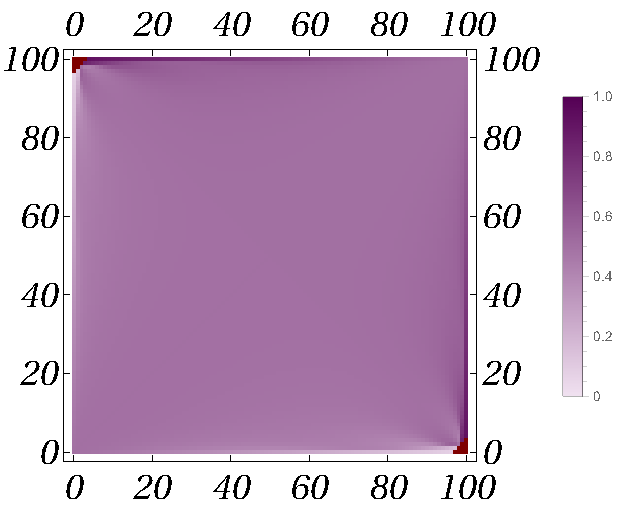
\includegraphics[width=\textwidth]{img/PB_Plot_4_100.pdf}
        \caption{\small \centering $P^*(K_A,K_B)$}
        \label{fig:BGame4__100_P}
    \end{subfigure}
    \hfill % space between images
    \begin{subfigure}[b]{0.3\textwidth}
        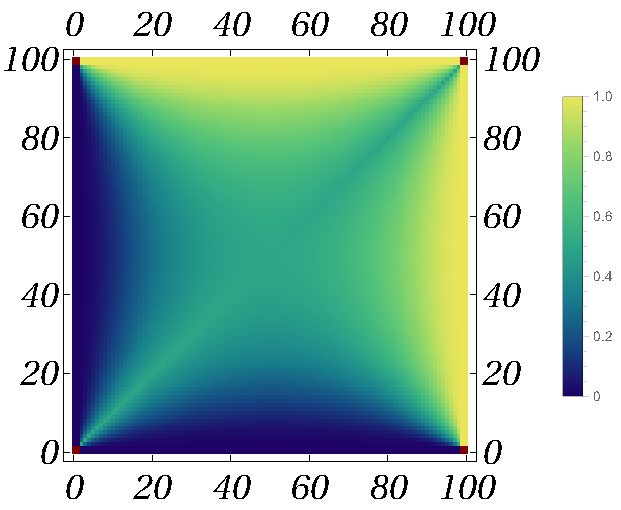
\includegraphics[width=\textwidth]{img/ppkB_Plot_4_100.pdf}
        \caption{\small \centering $p'^*_{k=2}(K_A,K_B)$}
        \label{fig:BGame4__100_ppk_2}
    \end{subfigure}
    \hfill % space between images
    \begin{subfigure}[b]{0.3\textwidth}
        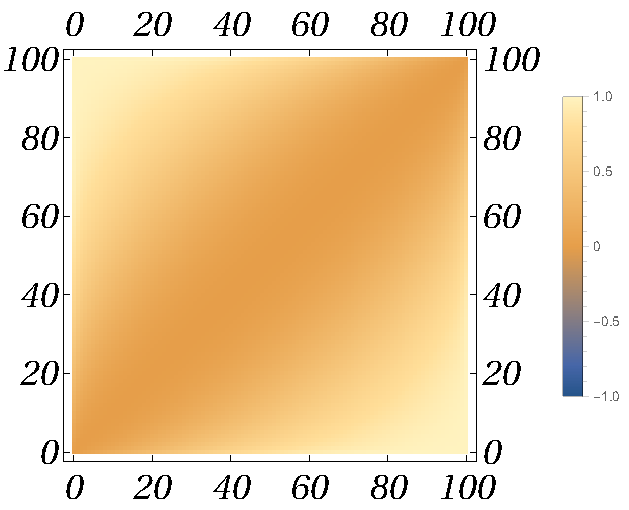
\includegraphics[width=\textwidth]{img/GB_Plot_4_100.pdf}
        \caption{\small \centering $G^*(K_A,K_B)/\log(2)$}
        \label{fig:BGame4__100_G}
    \end{subfigure}
    
    \caption{\small \centering \BG{N=4,K_A,K_B,M=100}}
    \label{fig:BGame4__100_PppkG}
\end{figure}
\end{frame}


\begin{frame}{Emerged Bayesian concepts}


\begin{columns}

\begin{column}{0.5\textwidth}
            
\begin{itemize}
    \item Bayes' rule 
    \item Exchangeabilit
    \item Shannon entropy
    \item Reference(-like) prior
    \item Emergence of probability distributions
    \item Interpretation of mixed strategies
\end{itemize}
        \end{column}

% Column 2    
\begin{column}{0.5\textwidth}
    \begin{figure}
    \centering
        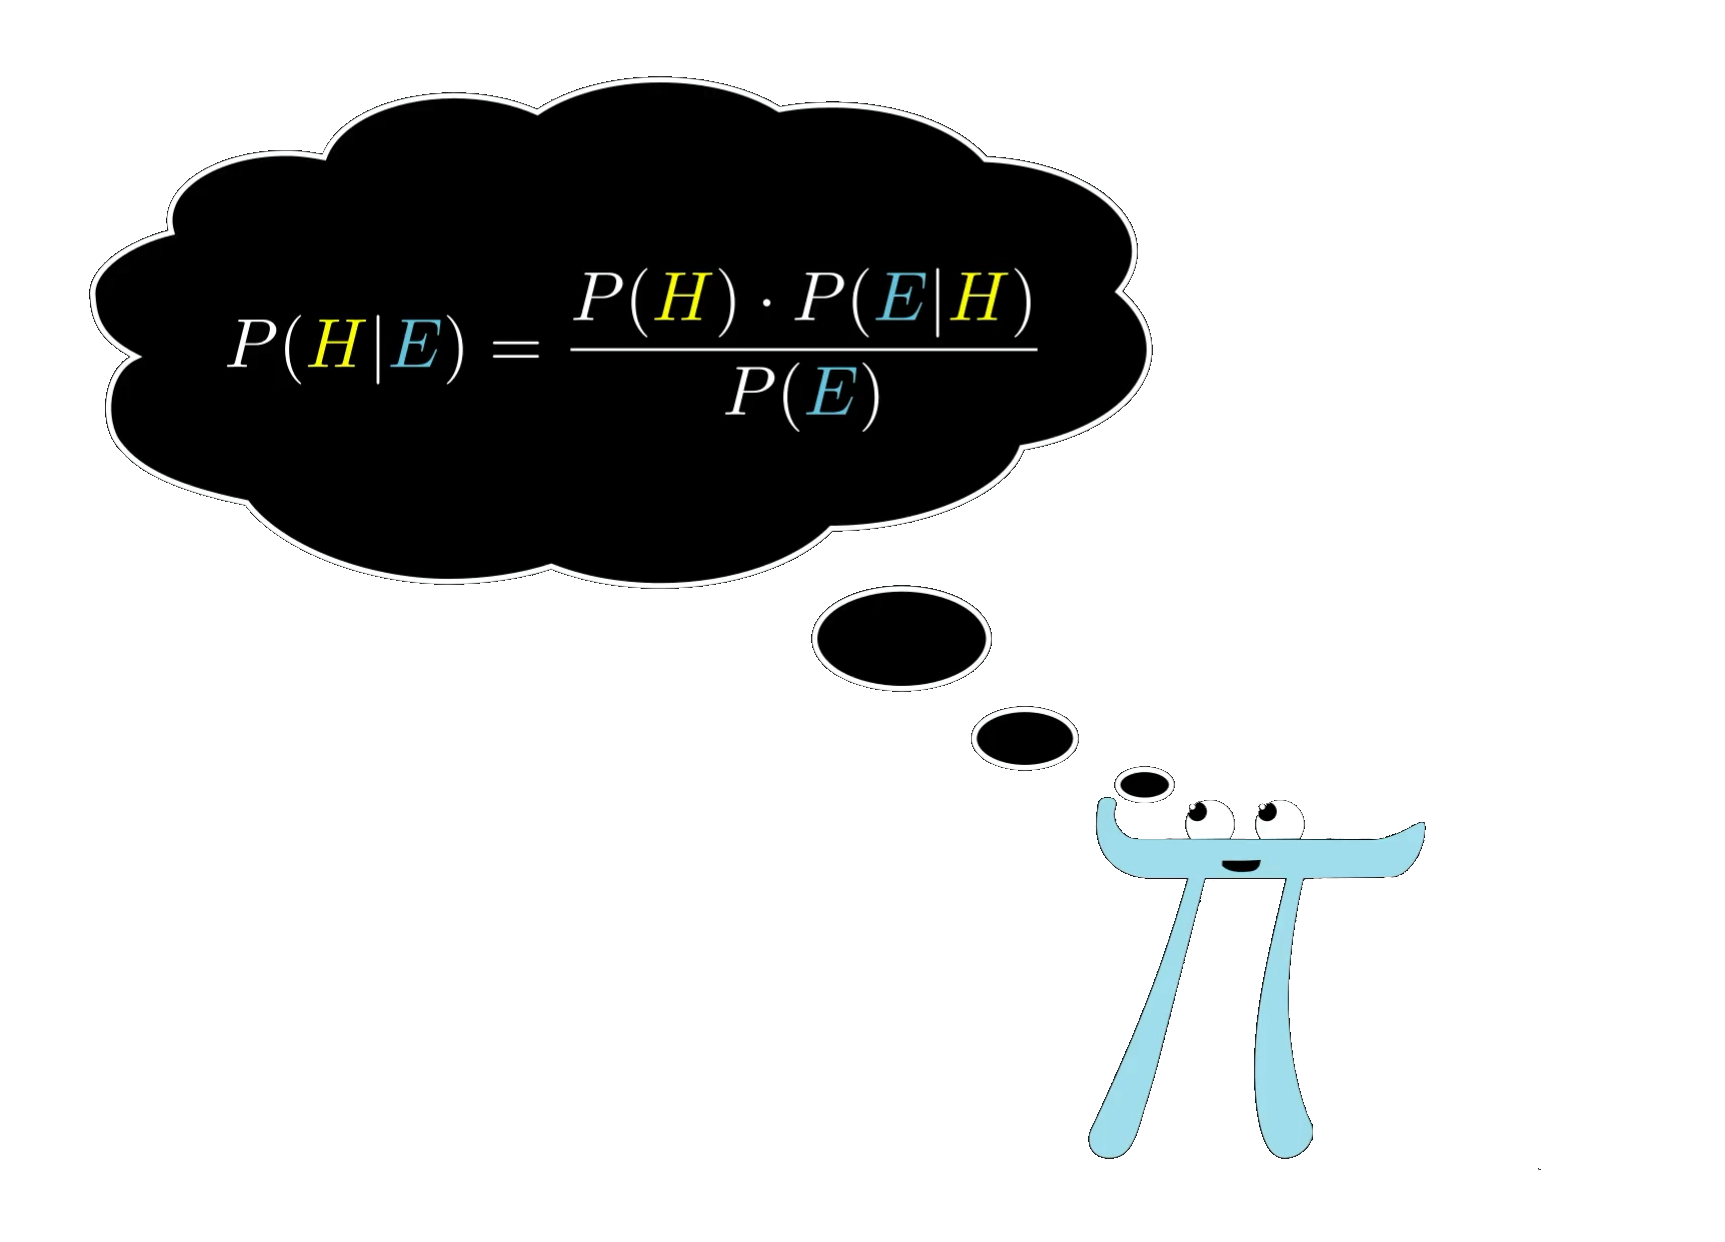
\includegraphics[width=\textwidth]{img/BlueBayes.png}
        \caption{\small \centering  Bayes' theorem by \href{https://www.3blue1brown.com/lessons/bayes-theorem}{3Blue1Brown}}
    \end{figure}
\end{column}
        

\end{columns}


\end{frame}

\section{Limiting cases}

\subsection{Binomial games}

\begin{frame}{Binomial games}

$M \to \infty$, while $K_A/M \to x_A \in (0,1)$ and $K_B/M \to x_B \in (0,1)$ \footnote{$x_A, x_B$ are similar fractions as mole fractions in chemistry.}.

This sequence of games will be denoted by:

\begin{equation}
    \lim_{\begin{smallmatrix} M \to \infty & \\ K_A/M \to x_A \\ K_B/M \to x_B \end{smallmatrix}} \textswab{Game}(N, K_A, K_B, M) = \overline{\textswab{Game}}(N, x_A, x_B)
\end{equation}

\begin{equation}
    \lim_{\begin{smallmatrix} M \to \infty & \\ K_A/M \to x_A \\ K_B/M \to x_B \end{smallmatrix}} \textswab{BGame}(N, K_A, K_B, M) = \overline{\textswab{BGame}}(N, x_A, x_B)
\end{equation}
    
\end{frame}

\begin{frame}{Examples}

    \begin{figure}[H]
    \centering
    \begin{subfigure}[b]{0.4\textwidth}
        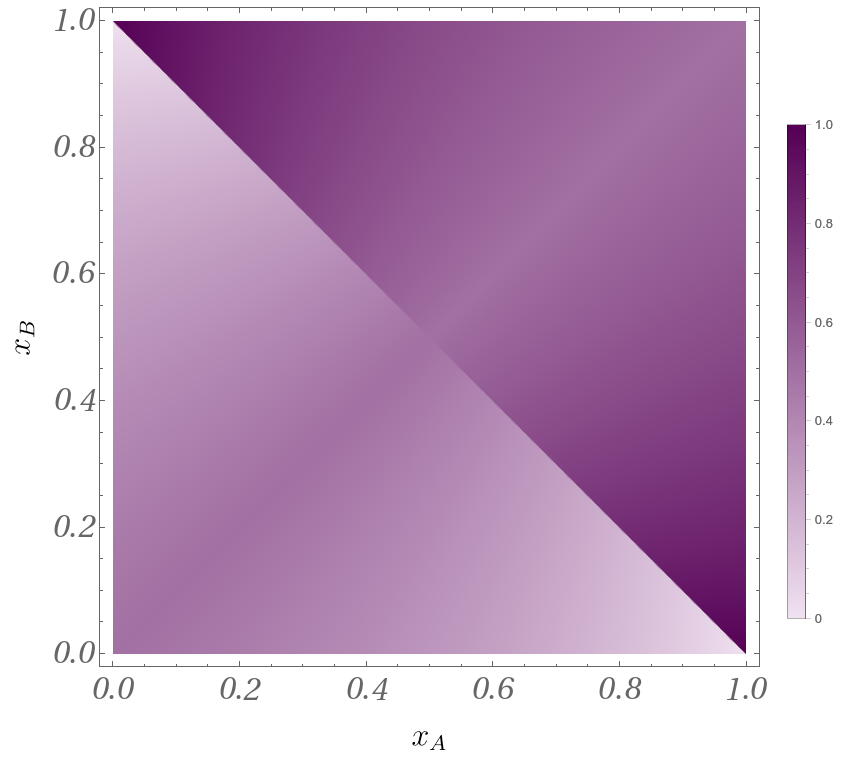
\includegraphics[width=\textwidth]{img/BinomialFisher_1.png}
        \caption{\small \centering \InfG{1,x_A,x_B}}
        \label{fig:PG_1}
    \end{subfigure}
    \hspace{0.05\textwidth} % space between images
    \begin{subfigure}[b]{0.4\textwidth}
        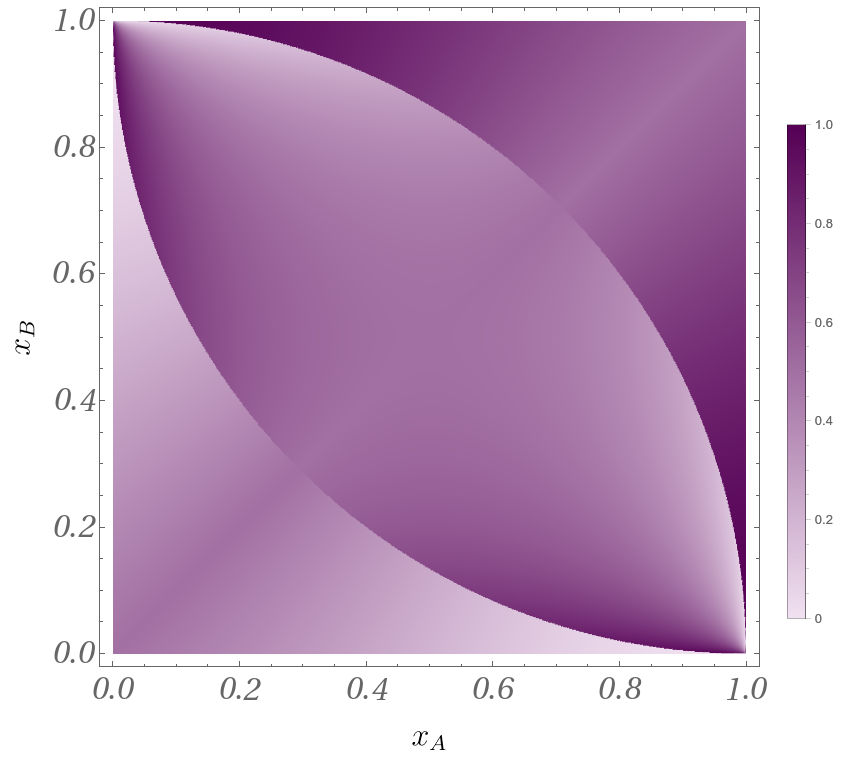
\includegraphics[width=\textwidth]{img/BinomialFisher_2.png}
        \caption{\small \centering \InfG{2,x_A,x_B}}
        \label{fig:PG_2}
    \end{subfigure}
    
    \caption{\small \centering $P^*(x_A,x_B)$ for Binomial Fisher games.}
    \label{fig:P_InfG_1_2}
\end{figure}

\end{frame}

\begin{frame}{Examples}

    \begin{figure}[H]
    \centering
    \begin{subfigure}[b]{0.4\textwidth}
        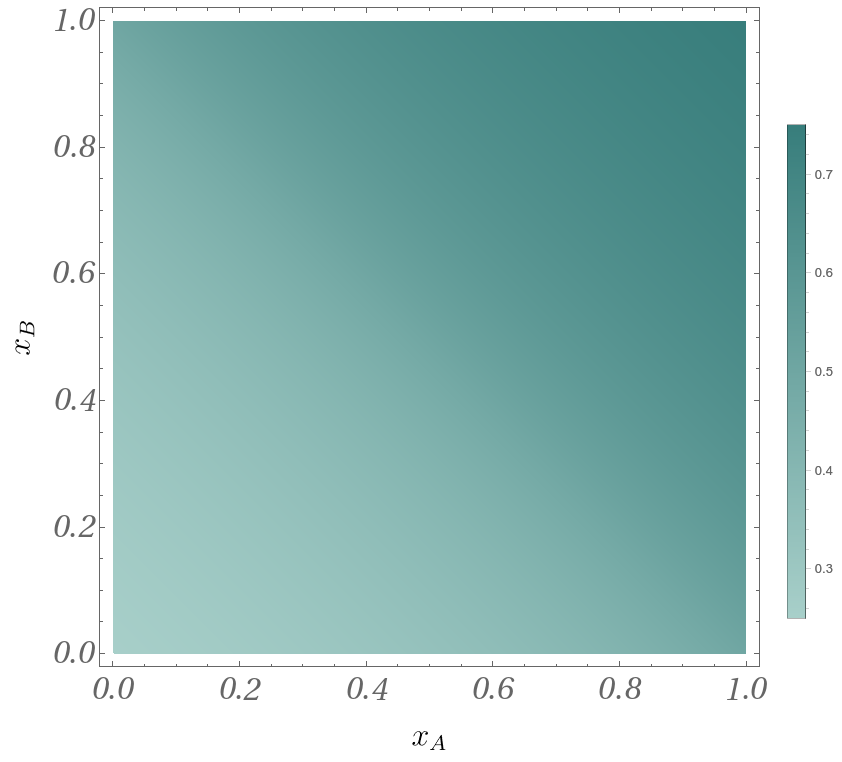
\includegraphics[width=\textwidth]{img/BinomialFisher_s_1.png}
        \caption{\small \centering \InfG{1,x_A,x_B}}
        \label{fig:sG_1}
    \end{subfigure}
    \hspace{0.05\textwidth} % space between images
    \begin{subfigure}[b]{0.4\textwidth}
        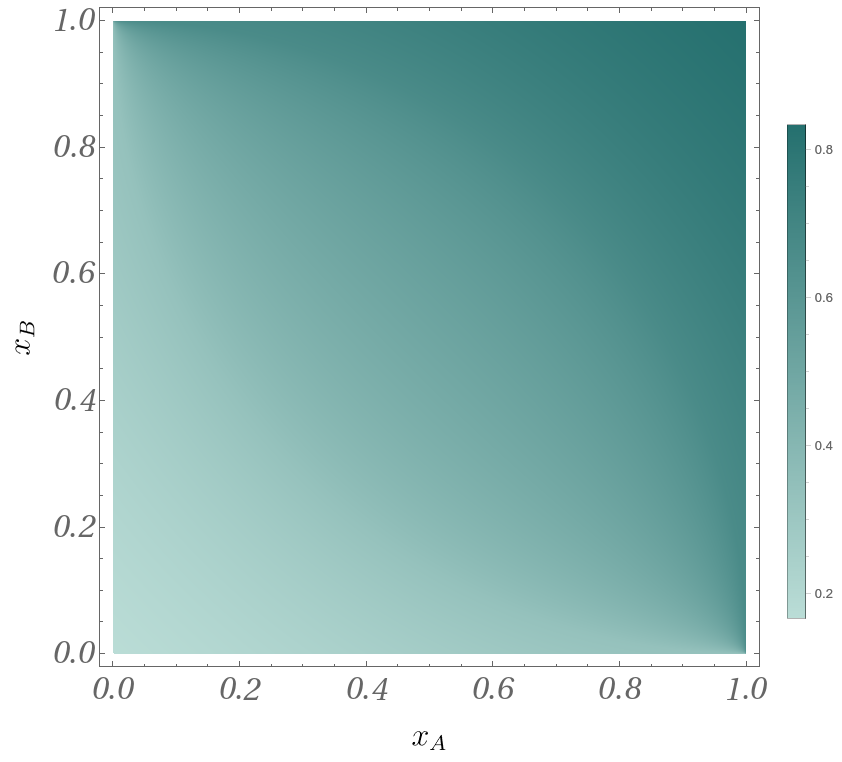
\includegraphics[width=\textwidth]{img/BinomialFisher_s_2.png}
        \caption{\small \centering \InfG{2,x_A,x_B}}
        \label{fig:sG_2}
    \end{subfigure}
    
    \caption{\small \centering $s^*(x_A,x_B)$ for Binomial Fisher games.}
    \label{fig:s_InfG_1_2}
\end{figure}
\end{frame}



\begin{frame}{Examples}

    
\begin{figure}[H]
    \centering
    \begin{subfigure}[b]{0.4\textwidth}
        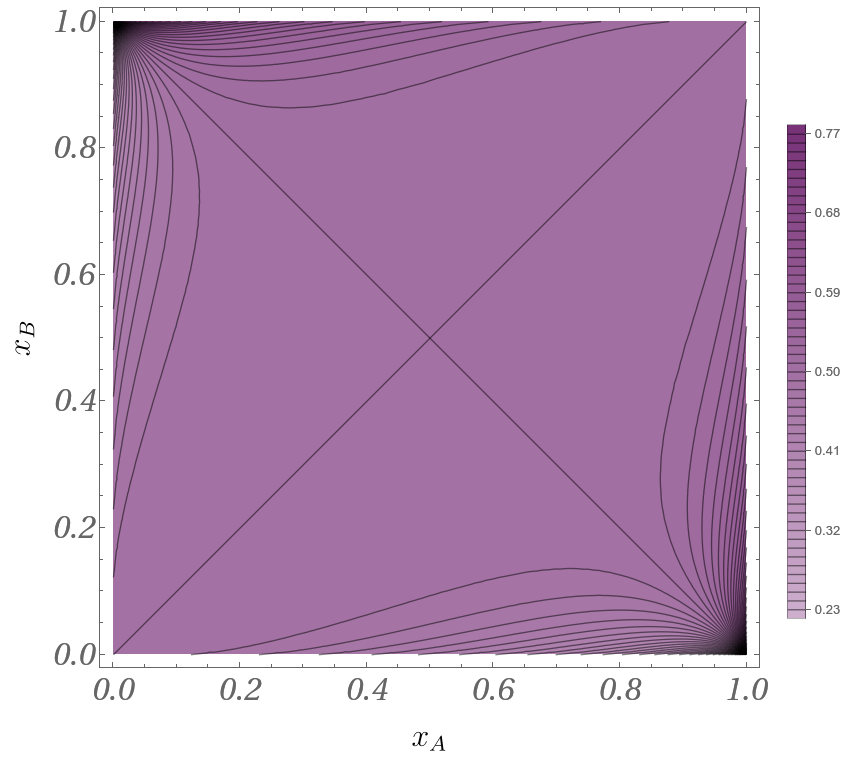
\includegraphics[width=\textwidth]{img/BinomialBayesian_1.png}
        \caption{\small \centering \InfBG{1,x_A,x_B}}
        \label{fig:PBG_1}
    \end{subfigure}
    \hspace{0.05\textwidth} % space between images
    \begin{subfigure}[b]{0.4\textwidth}
        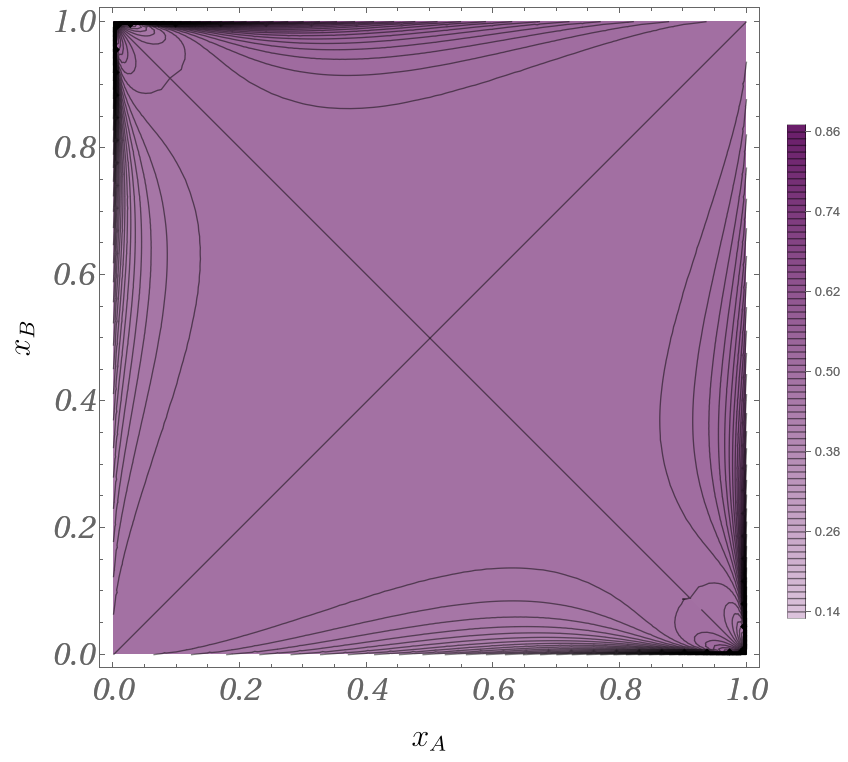
\includegraphics[width=\textwidth]{img/BinomialBayesian_2.png}
        \caption{\small \centering \InfBG{2,x_A,x_B}}
        \label{fig:PBG_2}
    \end{subfigure}
    
    \caption{\small \centering $P^*(x_A,x_B)$ for Binomial Bayesian games. Contour lines show $1\%$ difference.}
    \label{fig:P_InfBG_1_2}
\end{figure}

\end{frame}

\begin{frame}{Examples}

    \begin{figure}[H]
    \centering
    \begin{subfigure}[b]{0.4\textwidth}
        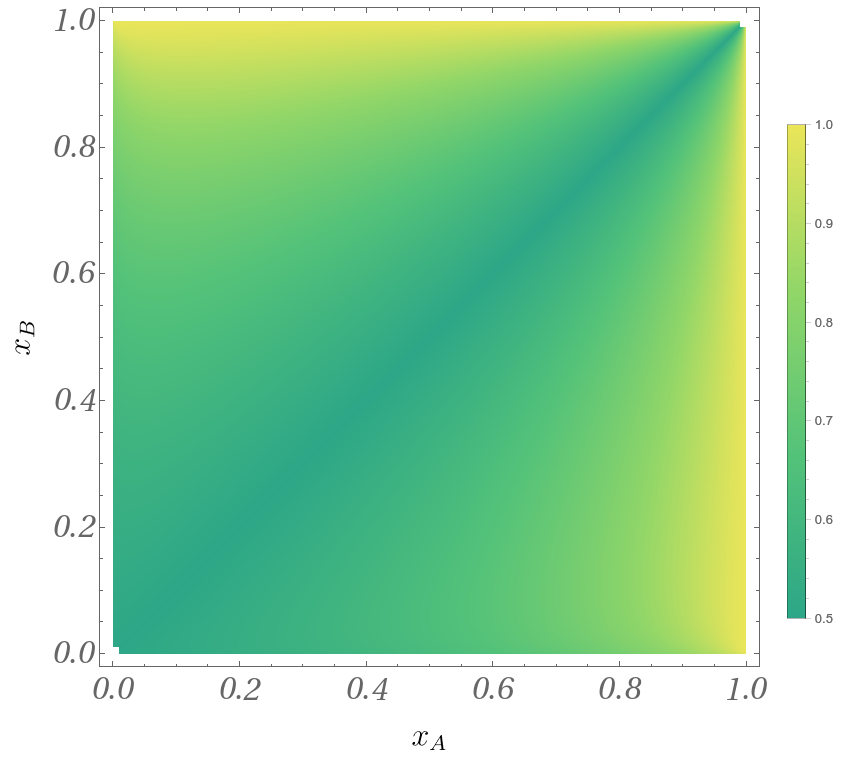
\includegraphics[width=\textwidth]{img/BinomialBayesian_ppk_1_0.png}
        \caption{\small \centering $k=0$}
        \label{fig:ppkBG_1_0}
    \end{subfigure}
    \hspace{0.05\textwidth} % space between images
    \begin{subfigure}[b]{0.4\textwidth}
        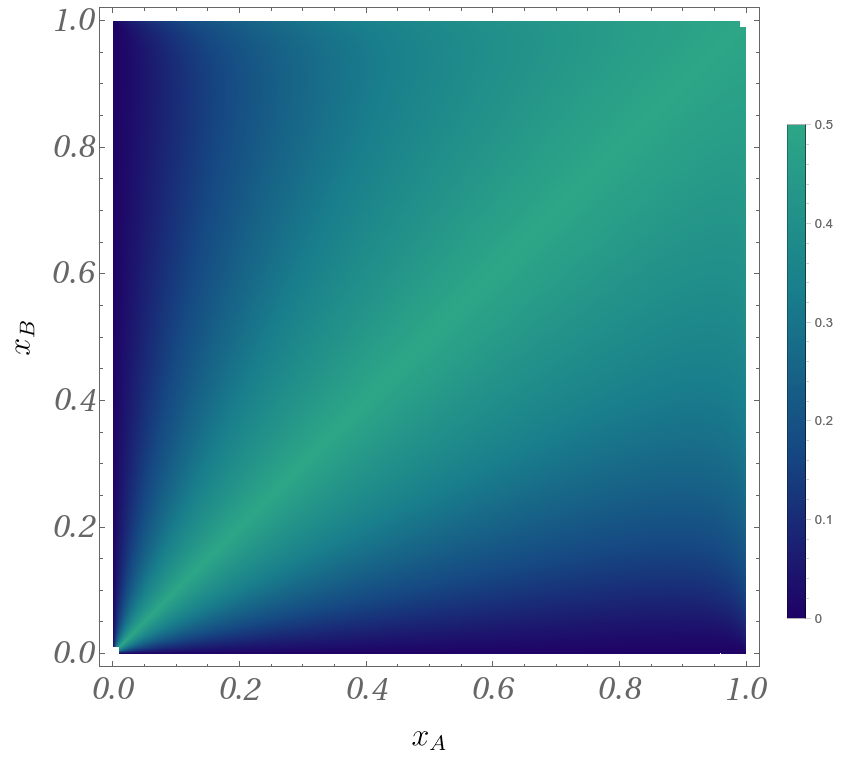
\includegraphics[width=\textwidth]{img/BinomialBayesian_ppk_1_1.png}
        \caption{\small \centering $k=1$}
        \label{fig:ppkBG_1_1}
    \end{subfigure}
    
    \caption{\small \centering $p'^*_k(x_A,x_B)$ for \InfBG{1,x_A,x_B}.}
    \label{fig:ppk_InfBG_1_01}
\end{figure}

\end{frame}

\begin{frame}{Examples}

    
\begin{figure}[H]
    \centering
    \begin{subfigure}[b]{0.3\textwidth}
        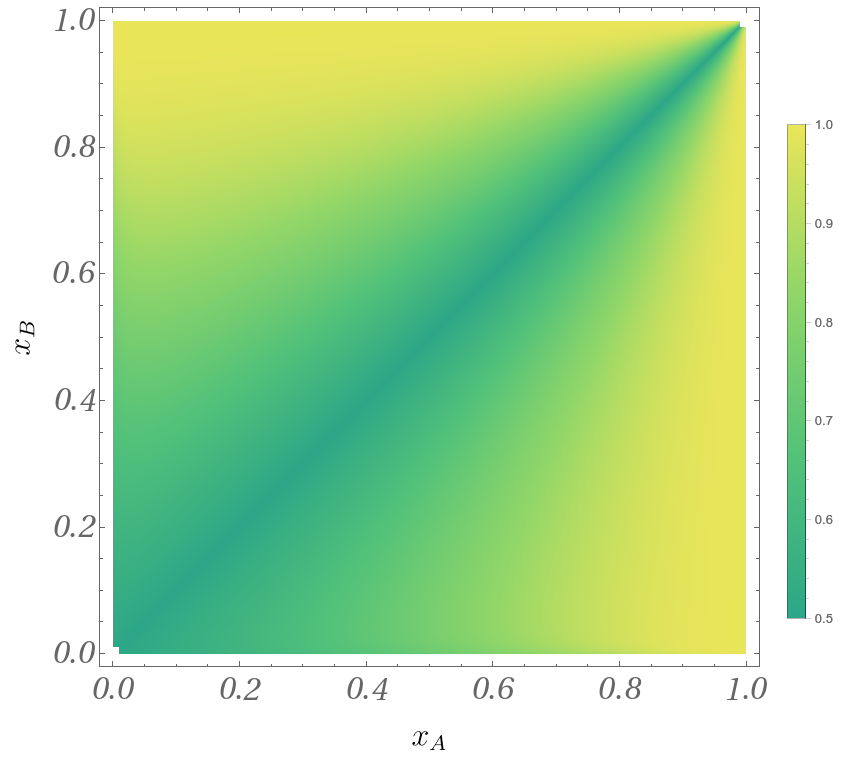
\includegraphics[width=\textwidth]{img/BinomialBayesian_ppk_2_0.png}
        \caption{\small \centering $k=0$}
        \label{fig:ppkBG_2_0}
    \end{subfigure}
    \hspace{0.01\textwidth} % space between images
    \begin{subfigure}[b]{0.3\textwidth}
        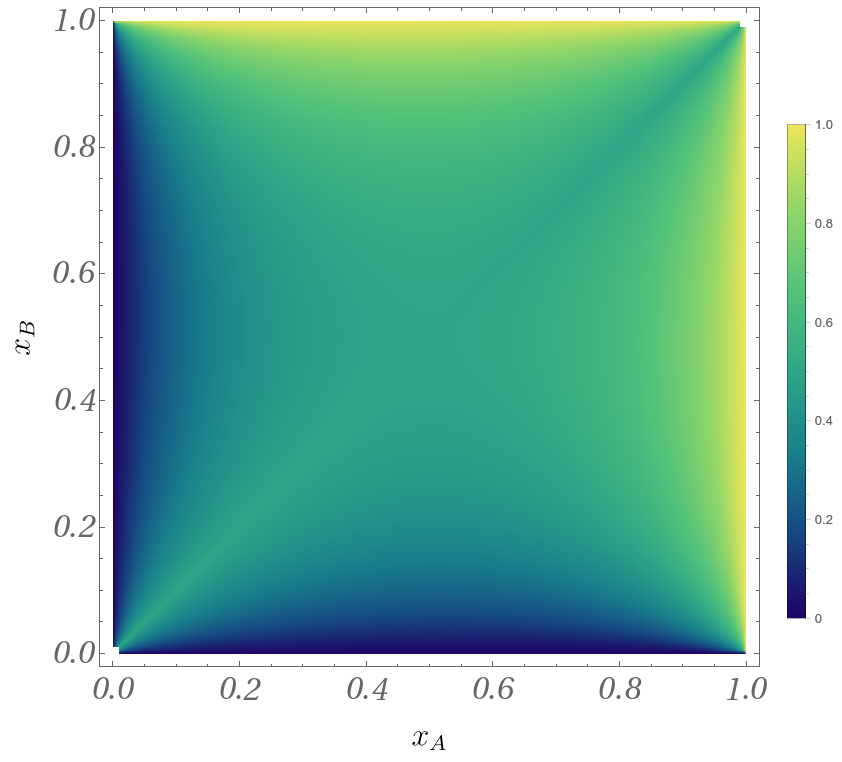
\includegraphics[width=\textwidth]{img/BinomialBayesian_ppk_2_1.png}
        \caption{\small \centering $k=1$}
        \label{fig:ppkBG_2_1}
    \end{subfigure}
    \hspace{0.01\textwidth} % space between images
    \begin{subfigure}[b]{0.3\textwidth}
        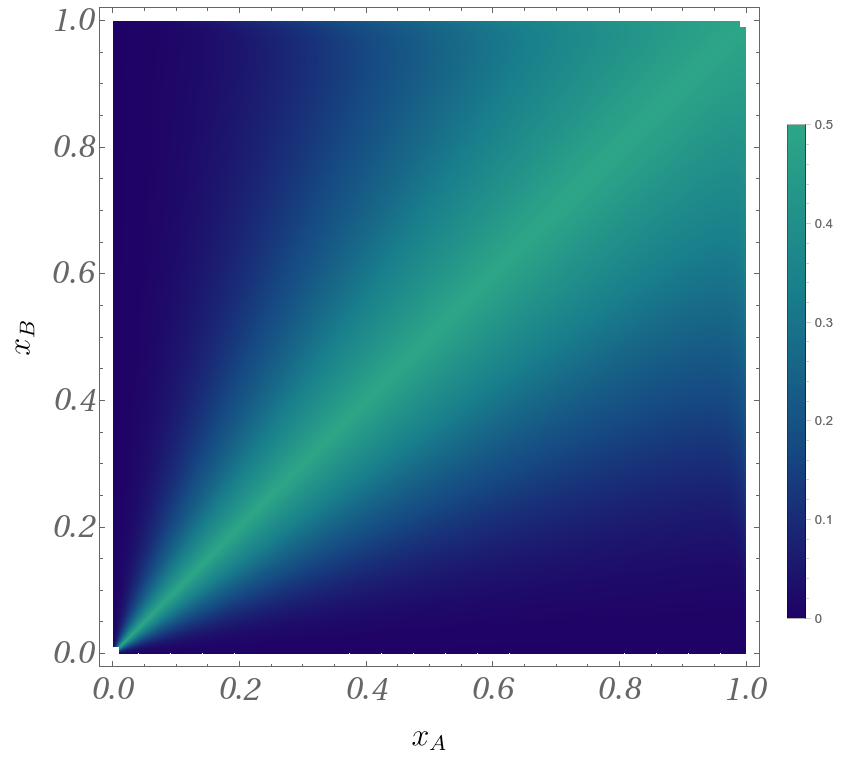
\includegraphics[width=\textwidth]{img/BinomialBayesian_ppk_2_2.png}
        \caption{\small \centering $k=2$}
        \label{fig:ppkBG_2_2}
    \end{subfigure}
    
    \caption{\small \centering $p'^*_k(x_A,x_B)$ for \InfBG{2,x_A,x_B}.}
    \label{fig:ppk_InfBG_2_012}
\end{figure}

    
\end{frame}

\subsection{$N \to \infty$ limit}

\begin{frame}{Limiting policies for $N \to \infty$}

    \begin{equation}
    x_0^*(x_A,x_B) = \frac{\log \left ( \frac{1-x_A}{1-x_B} \right )}{\log \left ( \frac{(1-x_A) x_B}{(1-x_B) x_A} \right )}
\end{equation}
    
    \begin{equation}
        \lim_{N \to \infty} s^*_N(x_A,x_B) = 
        s^*_\loopedsquare(x_A,x_B) =  x_0^*(x_A,x_B)
    \end{equation}
    meaning that for fixed $0 < x_A < x_B < 1$:
    
    \begin{equation}
        \lim_{N \to \infty} \frac{k^*_N + \nu^*_N}{N} =
        \lim_{N \to \infty} \frac{k^*_N}{N} =
        s^*_\loopedsquare =
        x_0^*
    \end{equation}
    
\end{frame}

\begin{frame}{Limiting policies for $N \to \infty$}


    \begin{figure}[H]
    \centering
    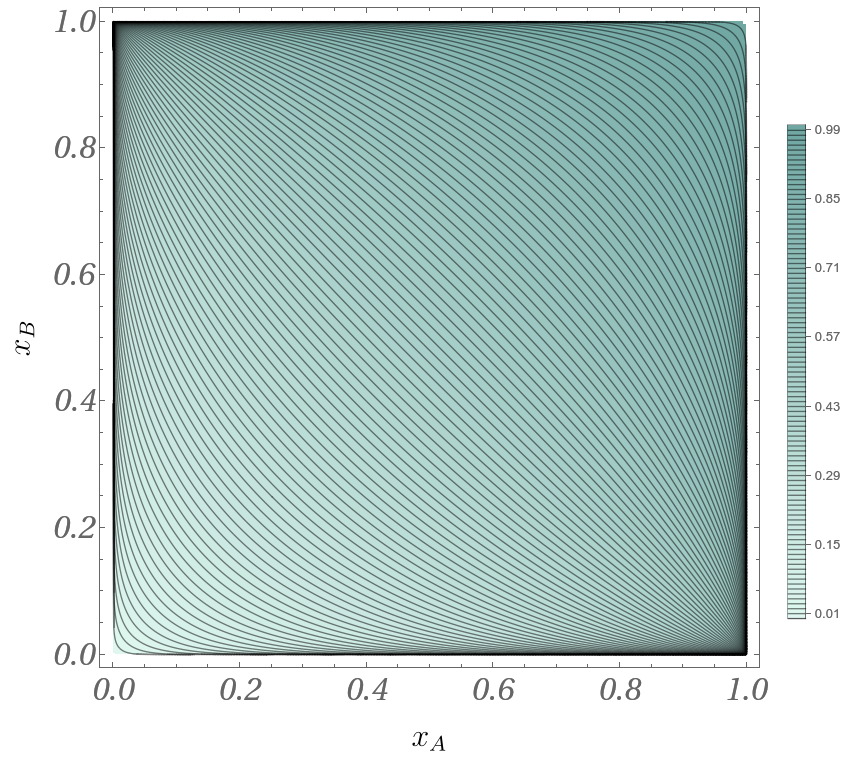
\includegraphics[width=0.55\textwidth]{img/FisherLimitPolicy.png}
    \caption{\centering \small Binomial Fisher policy limit $s^*_\loopedsquare(x_A,x_B)$. Contour lines show $1\%$ difference.}
    \label{fig:FisherPolicyLimit}
\end{figure}

\end{frame}

\begin{frame}[shrink=20]{Limiting policies for $N \to \infty$}

    \begin{equation*}
    P^\approx_\loopedsquare(x_A,x_B) = \frac{ \log \left ( \frac{(1-x_0^*) x_B}{(1-x_B)x_0^*}  \right )}{\log \left ( \frac{(1-x_A) x_B}{(1-x_B) x_A} \right )}, \quad
    x_0^*(x_A,x_B) = \frac{\log \left ( \frac{1-x_A}{1-x_B} \right )}{\log \left ( \frac{(1-x_A) x_B}{(1-x_B) x_A} \right )}
\end{equation*}

\begin{table}[H]
\centering
\begin{tabular}{|c|c|c|c|c|c|c|c|c|}
\hline
$x_A \backslash x_B$ & $20\%$ & $30\%$ & $40\%$ & $50\%$ & $60\%$ & $70\%$ & $80\%$ & $90\%$ \\
\hline
$10\%$ & 0.4761 & 0.4651 & 0.4598 & 0.4584 & 0.4604 & 0.4661 & 0.4772 & 0.5000 \\
$20\%$ &  & 0.4887 & 0.4832 & 0.4816 & 0.4833 & 0.4889 & 0.5000 & 0.5228 \\
$30\%$ &  &  & 0.4944 & 0.4928 & 0.4945 & 0.5000 & 0.5111 & 0.5339 \\
$40\%$ &  &  &  & 0.4983 & 0.5000 & 0.5055 & 0.5167 & 0.5396 \\
$50\%$ &  &  &  &  & 0.5017 & 0.5072 & 0.5184 & 0.5416 \\
$60\%$ &  &  &  &  &  & 0.5056 & 0.5168 & 0.5402 \\
$70\%$ &  &  &  &  &  &  & 0.5113 & 0.5349 \\
$80\%$ &  &  &  &  &  &  &  & 0.5239 \\
\hline
\end{tabular}
\caption{Binomial Bayesian limit prior approximation $P^\approx_\loopedsquare(x_A,x_B)$ up to 4 digits.}
\label{tab:BayesianPriorApprox}
\end{table}

\end{frame}

\begin{frame}{Bayesian game prior approximation for $N \to \infty$}


    \begin{figure}[H]
    \centering
    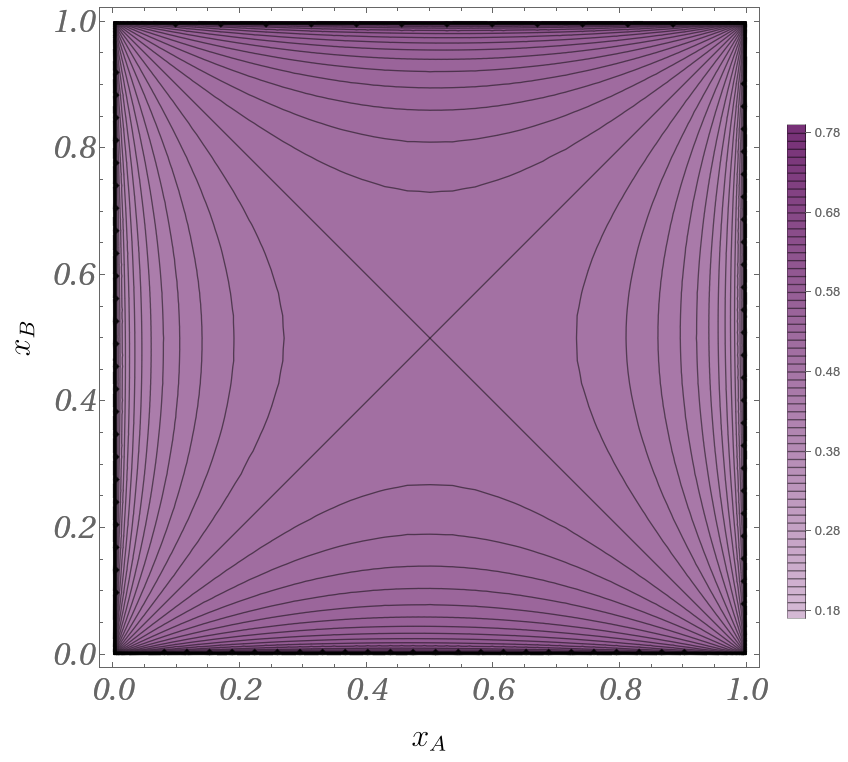
\includegraphics[width=0.55\textwidth]{img/BayesianPrior.png}
    \caption{\small \centering Binomial Bayesian limiting prior approximation $P^\approx_\loopedsquare(x_A,x_B)$. Contour lines show $1\%$ difference.}
    \label{fig:BayesianPriorApprox}
\end{figure}

\end{frame}

\begin{frame}{Numerical evidence}

    \begin{figure}[H]
    \centering
    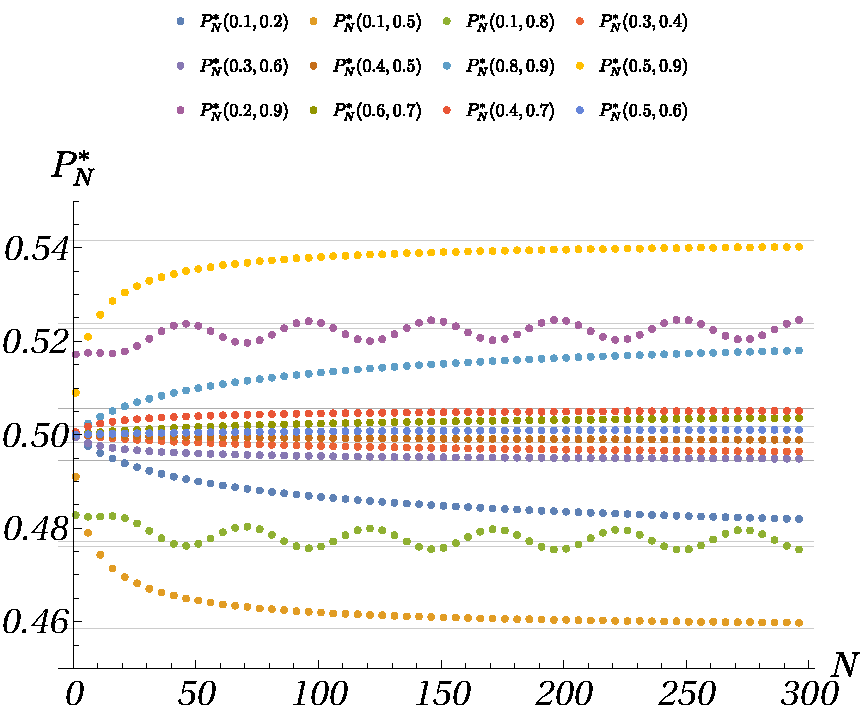
\includegraphics[width=0.7\textwidth]{img/Prior_Numerics.pdf}
    %\caption{}
    \label{fig:PriorNumerics}
\end{figure}
\end{frame}

\begin{frame}{Numerical evidence and Asymtotic expansion}

\begin{figure}[H]
    \centering
    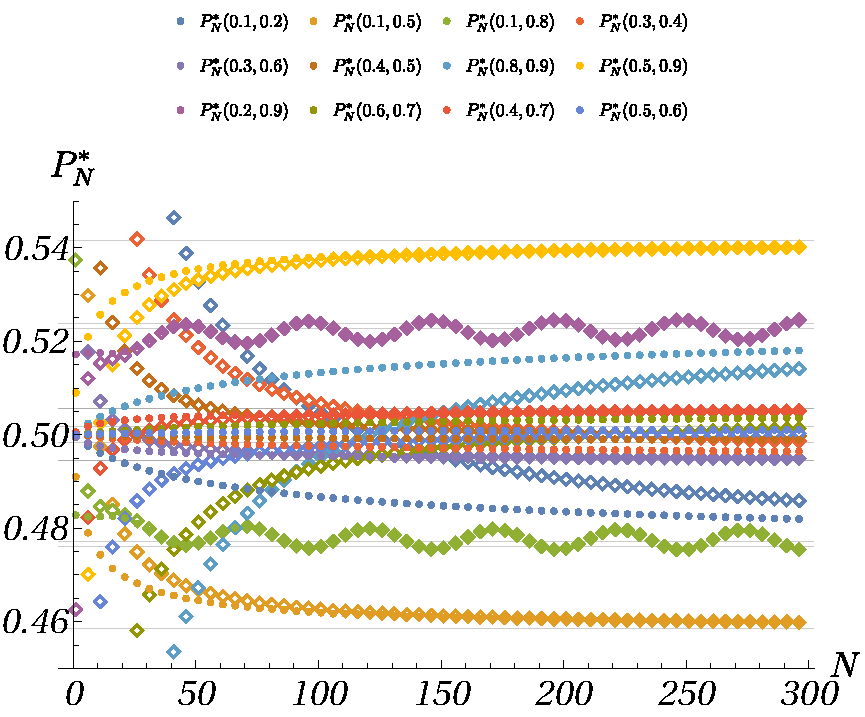
\includegraphics[width=0.7\textwidth]{img/Prior_Numerics_Asymptotics.pdf}
    %\caption{Numerically calculated $P^*_N(x_A,x_B)$ values marked by coloured dots ($\bullet$), and the values of first-order asymptotics $P^{*,(1)}_N(x_A,x_B)$ marked by coloured diamonds ($\diamond$).  
    %(Gridlines are placed at zeroth-order limiting prior approximations $P^\approx_\loopedsquare(x_A,x_B)$.)
    %}
    \label{fig:PriorNumericsAsymptotics}
\end{figure}

\end{frame}

\begin{frame}{First-order Asymptotic expansion of $P_N(x_A,x_B)$}

\begin{equation*}
    P^{*,(1)}_N(x_A,x_B) =
    \sigma \left (
    \vartheta^{*,\varphi_N(x_A,x_B)}_\loopedsquare(x_A,x_B) + \frac{1}{N} \sampi^{\varphi_N(x_A,x_B)}(x_A,x_B)
    \right )
\end{equation*}

where $\sigma(.)$ stands for the sigmoid function $\sigma(x) = 1/(1+e^{-x})$.

\begin{equation*}
    \varphi = 2 \pi N x_0^* \mod 2 \pi
\end{equation*}

For details see Appendix D in \href{https://arxiv.org/abs/2402.15892}{arXiv:2402.15892}

\end{frame}

\section{Statistical games}

\subsection{Statistical games}

\begin{frame}{}

\begin{definition}[Statistical game]
\label{def:StatisticalGame}

Same as \BG{N, K_A, K_B, M}, but with isoelastic utility function:

\begin{equation}
    u_\gamma(c) = \frac{c^{1-\gamma}-1}{1-\gamma}
\end{equation}
with relative risk aversion parameter $\gamma > 0, \gamma \ne 1$.

The above defined Statistical Game will be denoted as 
\SG{N, K_A, K_B, M, \gamma}.

\end{definition}

For arguments why are isoelastic utilities special, see Appendix~E in \href{https://arxiv.org/abs/2402.15892}{arXiv:2402.15892}

\end{frame}

\begin{frame}{}

    \begin{figure}[H]
    \centering
    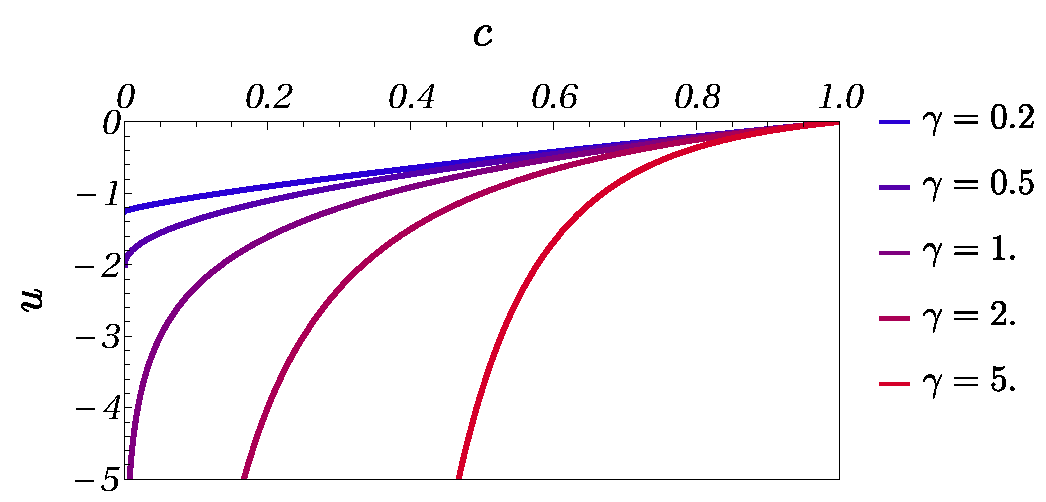
\includegraphics[width=0.9\textwidth]{img/u_gamma_c.pdf}
    \caption{\small \centering Isoelastic utility functions, for several relative risk aversion ($\gamma$) parameters: $u_\gamma(c)$.}
    \label{fig:IsoelasticUtility}
\end{figure}
\end{frame}

\begin{frame}{}


    \begin{figure}[H]
    \centering
    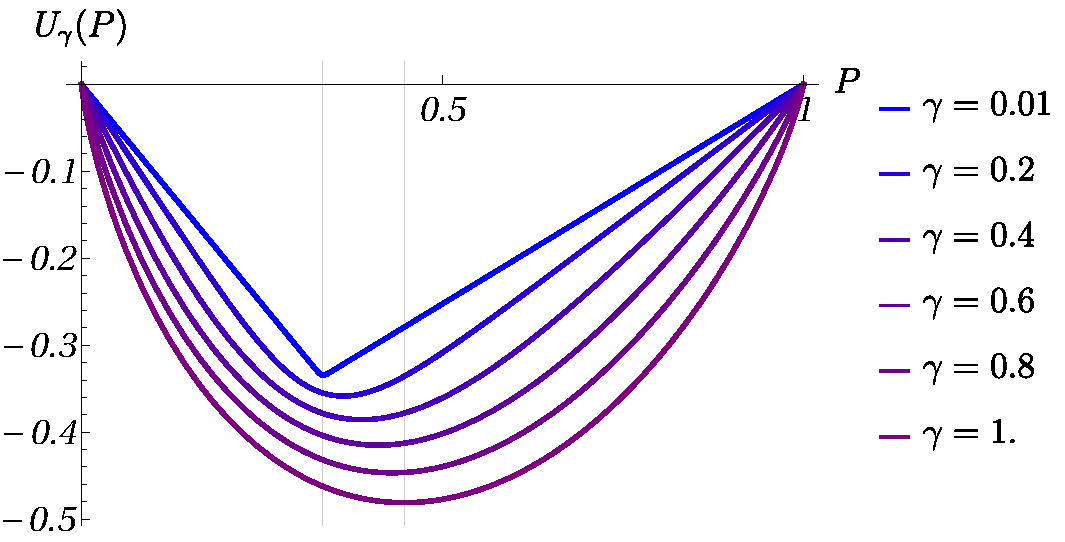
\includegraphics[width=0.8\textwidth]{img/EUP_1012_01.pdf}
    \caption{\small \centering Expected utility for \SG{N=1, K_A=0, K_B=1, M=2} as a function of $P$ for different $\gamma$ (relative risk aversion) values.
    (Vertical gridlines are placed at $1/3$ and $1/\sqrt{5}$ values.)}
    \label{fig:EUP_1012_01}
\end{figure}

\end{frame}

\begin{frame}[shrink=25]{}


    \begin{theorem}[Isoelastic equilibrium]
\label{thm:StatisticalGameEquilibrium}
\SG{N,K_A,K_B,M,\gamma} has a unique Nash equilibrium, in which:

\begin{equation}
    \label{thm:StatisticalEqHypergeom}
    p_k(A) = \frac{\binom{K_A}{k} \binom{M-K_A}{N-k}}{\binom{M}{N}}, \quad
    p_k(B) = \frac{\binom{K_B}{k} \binom{M-K_B}{N-k}}{\binom{M}{N}}
\end{equation}

\begin{equation}
\label{eq:ppkPgamma}
    p'_k(P) = \frac{\left ( P \ p_k(A) \right )^{1/\gamma}}{\left ( P \ p_k(A) \right )^{1/\gamma} + \left ( (1-P) \ p_k(B) \right )^{1/\gamma}}
\end{equation}

\begin{equation}
    p'^*_k = p'_k(P^*_\gamma)
\end{equation}

while $P^*_\gamma$ is the unique minimum of the expected utility:

\begin{equation}
    \label{eq:SGameExpectedUtility}
    U_\gamma(P) = P \ \left ( \sum_k p_k(A) u_\gamma(p'_k(P)) \right ) 
    + (1-P) \left ( \sum_k p_k(B) u_\gamma(1-p'_k(P)) \right )
\end{equation}

where the utility function for a given relative risk aversion $\gamma>0, \gamma \ne 1$ is:

\begin{equation}
    u_\gamma(c) = \frac{c^{1-\gamma}-1}{1-\gamma}
\end{equation}

\end{theorem}

\end{frame}

\begin{frame}{}


    \begin{figure}[H]
    \centering
    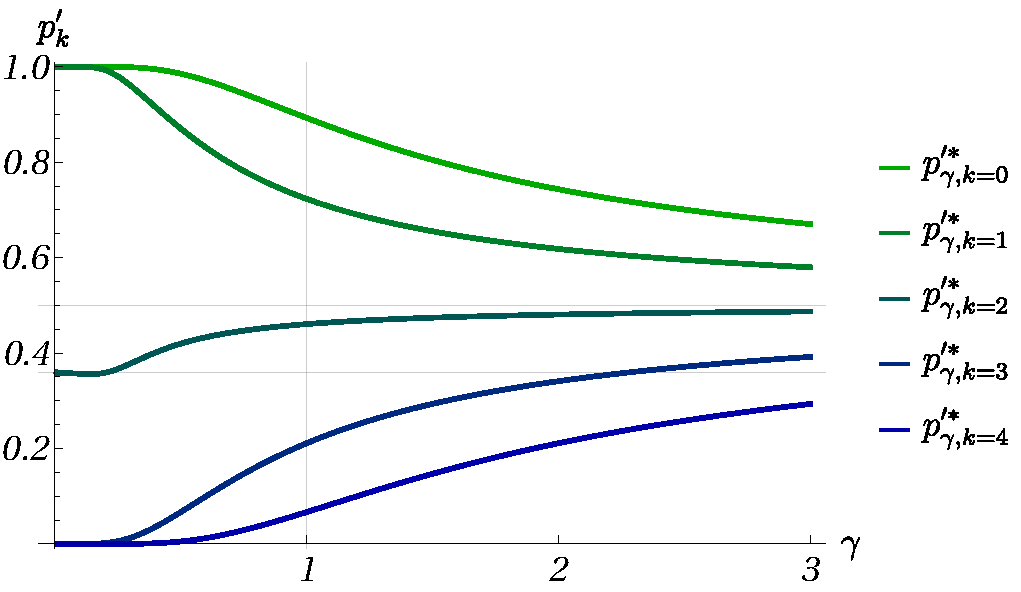
\includegraphics[width=0.8\textwidth]{img/pp_gamma_4_5_8_14.pdf}
    \caption{\small \centering Splitting strategies, $p'^*_{\gamma,k}$ for \SG{N=4, K_A=5, K_B=8, M=14} as a function of $\gamma$ (relative risk aversion parameter). Horizontal gridlines are placed at $\{1/2 , 14/39 \approx 0.359 \}$.}
    \label{fig:pp(gamma)_45814}
\end{figure}

\end{frame}

\subsection{Unification}

\begin{frame}{}

    \begin{theorem}
    The equilibrium strategies of a Statistical game \SG{N,K_A,K_B,M,\gamma} in the $\gamma \to 0$ limit can be mapped to the symmetric equilibrium strategies of a Fisher game \G{N,K_A,K_B,M} \footnote{if $\nu^* \ne 0$} with the following identification:
    \begin{equation}
        \lim_{\gamma \to 0} p'^*_{\gamma,k^*} = \nu^*
    \end{equation}
        
    \begin{equation}
        \lim_{\gamma \to 0} P^*_\gamma = P^*_0
    \end{equation}

    Where $(P^*_\gamma,\{p'^*_{\gamma,k}\})$ are the equilibrium parameters of 
    \SG{N,K_A,K_B,M,\gamma},
    while $(k^*,\nu^*,P^*_0)$ are the equilibrium parameters of 
    \G{N,K_A,K_B,M}.
    
\end{theorem}

\end{frame}

\begin{frame}{}

    \begin{figure}[H]
    \centering
    \includegraphics[width=0.9\textwidth]{img/AsymptoticExpasion_pp.pdf}
    \caption{\small \centering Illustration of $p'^*_{\gamma,k^*}$ and $p'^\times_{\gamma,k^*}$ for \SG{N=2,K_A=2,K_B=7,M=10}.}
    \label{fig:Asymptotic_pp}
\end{figure}

\end{frame}

\begin{frame}{Philosophical part }

Game-theoretical framework for Decision making in the face of Uncertainty:

\begin{itemize}
    \item Let us assume, the followings:
    \begin{itemize}
    \item An Agent can restrict the possible states of the world to a finite set. We will denote this set by $\Theta$ and call it the parameter set;
    \item The Agent can consider only a finite set of possible actions. The set of actions will be denoted by $\mathcal{A}$;
    \item Lastly, the Agent can associate utilities (or rewards) to all potential consequences, which depends both on her action and the possible state of the world. This function (in the finite representable by a matrix) will be denoted by $U: \mathcal{A} \times \Theta \mapsto \mathbb{R}$.
\end{itemize}
\end{itemize}

\end{frame}

\section{Philosophy \& Future work}

\begin{frame}{Philosophical part }

Under these assumptions, the game-theoretic framework for statistics would suggest the following strategy for the Agent:

\begin{itemize}
    \item Imagine that the unknown parameter $\theta \in \Theta$ has been chosen by an opponent whose utility function is the regret of the Agent;
    \item Determine the Nash equilibrium for such a two-player non-cooperative game;
    \item Adopt the equilibrium strategy of this imagined game to choose an action from the action set $\mathcal{A}$.
\end{itemize}

\end{frame}


\begin{frame}[shrink=15]{Future work and extension}

    \begin{columns}

\begin{column}{0.7\textwidth}
            
\begin{itemize}
    \item Assumptions about the unknown ($\mathghost$ vs. \hexacube{})
    \item Target of the Inference
    \begin{itemize}
        \item ``Platonian'' Inference (inferential risk)
        \item ``Aristotelian'' Inference (predictive risk)
        \item Data compression
        \item General
    \end{itemize}
    \item Correspondence with Bayesians and Frequentists
    \item Effective approximative numerical methods (Blahut–Arimoto algorithm)
    \item Generalizing Game Theory with a player representing uncertainty
    \item Using the concept in Reinforcement Learning
    \item Foundations of Statistical Physics
    \item Quantum metrology
    \item Universal Inductive Inference
    \item \dots
\end{itemize}

        \end{column}

% Column 2    
\begin{column}{0.3\textwidth}
    \begin{figure}
    \centering
        \includegraphics[width=0.9\textwidth]{img/logos/SagradaFamilia.pdf}
        \caption{\small \centering  \href{https://boutique.arte.tv/detail/sagrada-familia-le-defi-de-gaudi}{La Sagrada Família}, Antoni Gaudí: ``My client is in no hurry''.}
    \end{figure}
\end{column}
        

\end{columns}

\end{frame}


\begin{frame}{How is this related to AI?}

    \begin{columns}

% Column 2    
\begin{column}{0.5\textwidth}
    \begin{figure}
    \centering
        \includegraphics[width=0.85\textwidth]{img/MachineLearningMeme.jpg}
        \caption{\small \centering  \href{https://towardsdatascience.com/no-machine-learning-is-not-just-glorified-statistics-26d3952234e3}{No, Machine Learning is not just glorified Statistics}}
    \end{figure}
\end{column}

        % Column for the text
        \begin{column}{0.5\textwidth}
            \begin{itemize}
    \item Statistics $\to$ Game theory
    \item Frame: 
    \begin{itemize}
        \item Effective approximations and Scaling $\to$ Goal engineering
    \end{itemize}
    \item Machine Learning (ML) $\to$ Generative Adversarial Network (GAN)
    \item Artificial Intelligence (AI) $\to$ Better aligned AI, multi agent RL/AI 
\end{itemize}
        \end{column}

\end{columns}
\end{frame}

\begin{frame}{}

\centering \Huge
  {Thank you for your attention!}

    \vspace{0.85 cm}
    
  \pgfornament[height=0.85cm]{74}

    \vspace{0.85 cm}

    {\large
  \href{mailto:konczer.j@gmail.com}{konczer.j@gmail.com},
        \href{https://konczer.github.io/}{konczer.github.io}

        \href{https://arxiv.org/abs/2402.15892}{arXiv:2402.15892}
     }   
  
\end{frame}

\begin{frame}{}

\begin{figure}[H]
    \centering
    \includegraphics[width=0.7\textwidth]{img/QuestioningMind.png}
\end{figure}

\end{frame}


\end{document}